\def \ttb{\begin{ttfamily}}
\def \tte{\end{ttfamily}}
\def \na{\newcounter{alg}\setcounter{alg}{1}\arabic{alg}}
\def \ra{\setcounter{alg}{1}\arabic{alg}}
\def \sa{\stepcounter{alg}\arabic{alg}}
\def \line{\renewcommand{\baselinestretch}{1}}

\documentclass[10pt,oneside]{erc_bbk_report}
\usepackage[pdftex]{graphicx}
\usepackage{latexsym,erc_bbk,makeidx,epstopdf,amssymb,apalike,amsmath}
\usepackage{hyperref}
\usepackage{listings}
\usepackage{setspace}

%\usepackage{yfonts}
%\usepackage{helvet} % Helvetica as \ sfdefault
%\usepackage[T1]{fontenc}
%\usepackage{textcomp}
%\renewcommand{\familydefault}{\sfdefault }

%\usepackage{pxfonts} % Also loads Helvetica and PXTT
%\usepackage[T1]{fontenc}
%\usepackage{textcomp}

%\usepackage{bera}
%\usepackage{kerkis}

%\usepackage[T1]{fontenc}
%\usepackage[math]{kurier}

%\usepackage[T1]{fontenc}
%\usepackage{txfonts} % Also loads Helvetica and TXTT
%\usepackage{textcomp}\begin{center}

\usepackage{epstopdf}

\makeindex

\title{An Investigation into Price Surfaces for Credit Derivatives} 

\author{
Ethan Richard Collopy
}

\date{29 August 2008}  

\newcommand{\avec}[1]{\ensuremath{#1_1, \ldots, #1_n}}
\newcommand{\angavec}[1]{\ensuremath{\langle #1_1, \ldots, #1_n \rangle}}

\includeonly{abstract/abstract,contents/contents,introduction/symbol-index,introduction/introduction,review/review,investigation/investigation,conclusion/conclusion,exp_meth/exp_meth,code/code}

\begin{document}         

%\sfdefault
%\fontfamily{maksf}
%\usefont{U}{yinit}{m}{n}
%\lstset{language=Pascal}

\pagenumbering{arabic}

\maketitle 
%\bibliographystyle{alpha}
\bibliographystyle{apalike}

\newtheorem{theorem}{Theorem}[section]
\newtheorem{corollary}[theorem]{Corollary}
\newtheorem{lemma}[theorem]{Lemma}
\newtheorem{proposition}[theorem]{Proposition}
\newtheorem{definition}{Definition}[section]
\newtheorem{algorithm}{Algorithm}
\newtheorem{example}{Example}[section]


\include{abstract/abstract}
{\setlength{\baselineskip}{15pt}
\tableofcontents
\listoffigures
\listoftables
}

%\chapter*{Symbol Index}\label{chap:symbol}
    
\begin{symbolindex}

{\renewcommand{\baselinestretch}{1}
\small\normalsize
\begin{tabbing}
\hspace*{4cm}\=\kill \\
{\bf Symbol} \>        {\bf Meaning}\\
\\
NPV \> 		 Net Present Value\\
$K_L$ \> 		 Tranche Attachment point \\
$K_U$ \>  		 Tranche Detachment point \\
$F (\cdot)$ \> Cumulative Distribution Function \\
$F^{-1} (\cdot)$ \> Inverse Cumulative Distribution Function \\
$\Phi (\cdot)$ \> Cumulative Standard Normal Distribution Function \\
$\Phi^{-1} (\cdot)$ \> Inverse Cumulative Standard Normal Distribution Function \\
$w$		\>	Factor Sensitivity, square root of correlation \\
LGD	\>		Loss Given Default, equal to 1 - R (Recovery Rate) \\
PD	\>		Probability of Default \\
PS	\>		Probability of Survival \\
R	\>		Recovery Rate \\
FTD \>		First To Default \\
NTD \>		$N^{th}$ To Default \\
CDO	\> 		Collateralised Debt Obligation \\
CDS \>		Credit Default Swap \\
LHP \>		Large Homogenous Portfolio \\
bps \>		Basis Points, equivalent to one hundredth of a percent \\
T	\>		Time to maturity \\
	
\end{tabbing}

}


\end{symbolindex}


\chapter{Introduction}\label{chap:intro}\index{Introduction}


\medskip

In this dissertation we will investigate Credit Derivative Pricing Surfaces. We will
review the pricing mechanisms for these products and survey the current state of the art.   
In Chapter~\ref{chap:review} we review the credit derivatives market, introduce various credit derivatives products.  We attempt to refer to the 2007 Credit Crisis where appropriate as this is of direct consequence to the Credit Derivative marketplace. 

Who seeks to use Credit Derivatives and transfer credit risk? \cite{Gib2007} details the type of counterparty within credit derivative deals with the largest category of buyers being reporting dealers. \cite{Gib2007} also discusses the three market participants for credit derivatives, namely, commercial banks, investment banks, and investors.  Commercial banks seek to manage their risk exposure. For this they might use a single name CDS to diffuse credit risk of an issuer with whom they have significant exposure.   
An Investment bank would use credit derivatives to manage the credit risk of underwriting securities before it sells them to market, for example in the warehousing of a number of mortgage loans in the run up to securitisation. From 2004 CDSs on asset backed securities grew to \$125 billion in 2007 and these allowed underwriters to buy credit protection on these warehoused MBS deals. Finally, investors will purchase credit derivatives with many different strategies ranging from buy-and-hold (pension funds) to active trading (hedge funds), though even these distinctions can be vague.  

The International Swaps and Derivatives Association (ISDA) 2007 year-end survey of the over-the-counter derivatives market stated that credit default swaps (CDS), including single-name CDS, baskets and portfolios of credit and index trades, was the fastest growing asset class. The notional amount outstanding of CDSs increased 81 percent over the previous year to \$62.2 trillion from \$34.5 trillion at year-end 2006.\footnote{Source: http://www.securitiesindustry.com/news/22270-1.html}


\section{Credit Derivative Products}

The Credit Default Swap (CDS) is the most widely traded Credit Derivative. It is a bilateral contract which provides insurance against the default of a particular issuer \cite{Sch2003}. The buyer (of protection) makes periodic payments to the seller (of protection) until either the CDS maturity date or a default event occurs.  CDS contracts can be priced using standard risk neutral procedures, detailed in section~\ref{subsec:rnpricing}.

Credit Derivatives can essentially be demarcated into two categories; single and multi-name instruments. Single name instruments include CDSs and total return swaps whereas multi-name instruments include FTDs, NTDs and CDOs, where payment is based on the first or nth to default within a group of issuers or seniority based claims on a debt portfolio, respectively. CDOs can be synthetic or cash based. Synthetic CDOs, constructed from a portfolio of CDSs, now dominate the market over cash CDOs, constructed from loans and bonds which were more popular in the 90s. In Chapter~\ref{chap:review} we detail the pricing methodologies for those products upon which we conduct simulations in Chapter~\ref{chap:study}.  Additionally $CDO^2$s (CDO-squareds) are now an important part of the CDO market where the underlyings are themselves CDO tranches.


\section{The Credit Indices}

In June 2004 the first CDS indices were launched, these were iTraxx
in Europe (iTraxx.Europe) and Asia (iTraxx.Asia) and CDX in North America (CDX.NA). These indices represent the
average CDS premiums of the 125 most liquid investment grade credits.
Their values are calculated daily with the publically listed 
index composition recreated twice a year, providing liquidity for much of the credit derivatives market. Other indices include iTraxx Europe HiVol, a 30-entity index which trades those names with the largest spreads from the iTraxx Europe index, specific Sector based indices, such as Telecoms and Energy (25 entities each), and iTraxx Europe Crossover consisting of 50 sub investment grade names.  On each index multiple tranches are traded at a number of different maturities, principally 3, 5, 7, and 10 years.

{\begin{table}[ht]
\begin{center}
\begin{tabular}{||c|c|c|c|c|c||}
\hline \bf{Tranche} & \bf{$K_L - K_u$ \%} & \bf{5-year} & \bf{5-year Delta} & \bf{10-year} & \bf{10-year Delta} \\ 
\hline Equity & 0-3 \% & 500 + 31.01\% & 6.50 & 500 + 42.66\% & 4.00\\ 
\hline Junior Mezzanine & 3-6 \% & 351.10 & 3.75 & 549.40  & 4.25 \\ 
\hline Senior Mezzanine & 6-9 \% & 215.0 &  2.50 & 311.16 & 3.00 \\ 
\hline Senior & 9-12 \% & 136.10 &  1.70 & 185.75 & 2.15 \\ 
\hline Super Senior & 12-22 \% & 66.40 &  0.75 & 92.23 & 1.10 \\ 
\hline 
\end{tabular} 
\end{center}
\caption{\label{table:31Jul08}Spreads on the iTraxx EUR Series 9 IG tranches for 31 July 2008, source: \it{www.creditfixings.com}}
\end{table}
}

Within CDOs Portfolio loss is separated into tranches with each tranche categorised based on an attachment point and a detachment point.  Table~\ref{table:31Jul08} presents some iTraxx spread values where a Tranche having a value of, say, 6-9 \% has an attachment point of 6\% and a detachment point of 9\%. The Equity tranche is quoted as an upfront with a fixed 500bps spread and a percentage quote of the notional. The Delta values in Table~\ref{table:31Jul08} measure the relative size a position in the underlying index that has the same sensitivity to a small movement in the index spread as the tranche.  This can be viewed as the risk of the tranche relative to a position in the index and so we are able to compare the riskiness of tranches using these Delta values \cite{Gib2007}.  


\section{The Credit Crisis of 2007-8}\index{Credit Crisis}

\begin{figure}
\centerline{\scalebox{0.5}{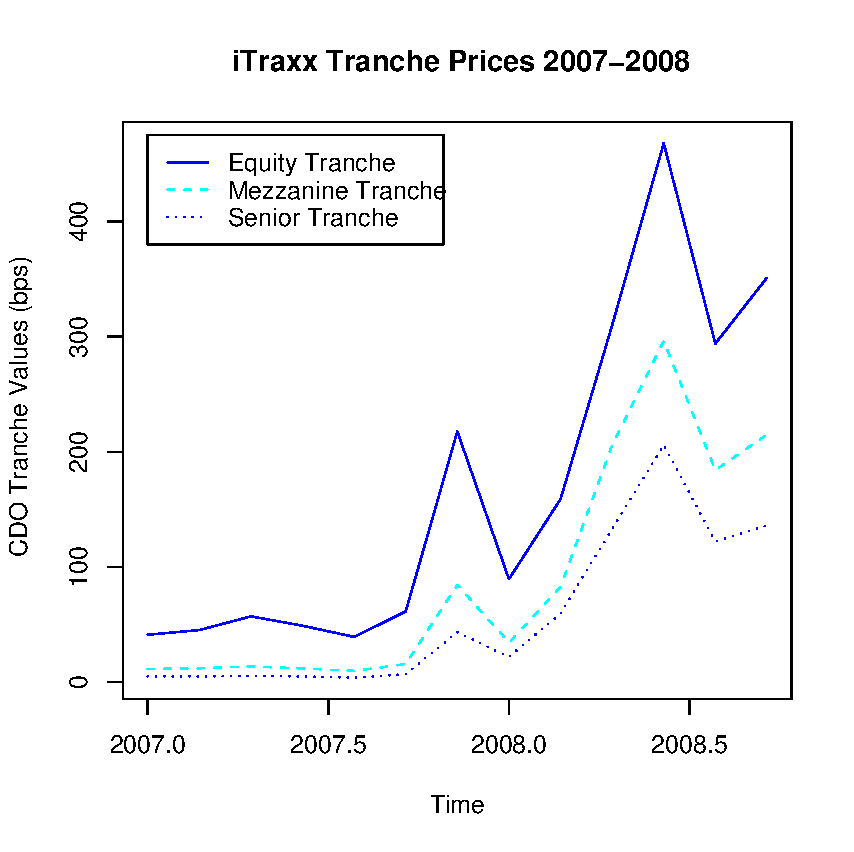
\includegraphics{pictures/iTraxxSpreads.pdf}}}
\caption{\label{table:trancheSpread}Changing Spreads on iTraxx.Europe index tranches from 01 Jan 2007 to 31 July 2008, source: \it{www.creditfixings.com}}
\end{figure}


As we can see from Figure~\ref{table:trancheSpread} the large jump in spreads occurred between June and July 2007 at the initiation of the credit crisis.  This followed reports on the 20th June that two Bear-Stearns managed hedge funds invested in securities backed by subprime mortgage loans were close to being shut down followed by, on the 10th July 2007, S \& P placing \$7.3 billion worth of 2006 vintage ABSs backed by residential mortgages on negative ratings watch and Moody's downgrading \$5bn worth of subprime mortgage bonds. Consequently, on the 11th July Moody's put 184 mortgage-backed on downgrade alert.

\cite{Green2005} presciently stated that "some observers ... are concerned that banks' efforts to lay off risk using credit derivatives may be creating concentrations of risk outside the banking system that could prove a threat to financial stability. A particular concern has been that, as credit spreads widen appreciably at some point from the extraordinarily low levels that have prevailed in recent years, losses to nonbank risk-takers could force them to liquidate their positions in credit markets and thereby magnify and accelerate the widening of credit spreads." It is standard practice for the originator of a CDO to retain the equity tranche. This is usually a bank intending to signal the riskiness of a deal whilst also serving to ensure prospective buyers that it will monitor credit payments.  \cite{Eli2006} notes that major banks do hold significant positions in the deals they construct and this is obviously a key factor in the losses suffered by these banks in the year 2007-2008.


\section{Outline \& Goals of this Report}\index{Outline}

In chapter~\ref{chap:review} we introduce and review Credit Derivatives, focussing on $N^{th}$-to-default Basket Swaps (NTDs) and Collateralised Debt Obligations (CDOs) and detail the prime risk-neutral mechanisms for pricing these products. Chapter~\ref{chap:study} details the practical investigation of this work whilst Chapter~\ref{chap:conclusion} concludes and attempts, and no more than that, to put into context the pricing issues with the market as seen over the period from June 2007 to August 2008.  Simulations for this report were implemented in the S programming language and executed on R 
(\url{http://www.r-project.org})
and S-plus (\url{http://www.insightful.com}) systems. Data was obtained from a number of sources, principally {\em Datastream} and \url{http://www.creditfixings.com}.

\chapter{An Introduction to Credit Derivatives}\label{chap:review}

The aims of this chapter are to provide the requisite
background to be able to understand how the key credit derivative instruments are used and priced. We survey many of the recently developed extensions to standard credit derivative pricing. We look at the introduction of default risk into option pricing \cite{JS1987}.
Credit Derivatives are financial securities that facilitate the transfer of credit risk from one agent to another. A periodic or upfront fee is paid by an agent in return for a structured payment should one of the underlying reference firms default.  Default can be outright bankruptcy or debt restructuring. Ratings data provided by the ratings agencies\footnote{Moody's KMV, S \& P, and Fitch amongst others} allows buyers and sellers to gauge the potential for either ratings changes or default.

\section{A Review of Credit Risk}\label{sec:cred_review}
\index{Credit Risk! Review}

\subsection{Model Risk}

Model Risk is the risk associated with using an inadequate model \cite{hs2002}. Model risk is amplified for CDOs as there can be errors in modeling both returns from entities and the relationships between entities \cite{bv2005}.  We also discuss the risks associated with Monte Carlo simulations in Appendix~\ref{subsec:accuracy}.

\subsection{What is Credit Risk?}\index{Credit Risk}

We begin with some definitions that will motivate credit based instruments.

\begin{definition}[Credit Risk]
\begin{rm}
is the risk due to uncertainty in a counterparty's ability to meet its obligations. Credit risk covers many different types of obligations from loans to complex derivative deals. 
\end{rm}
\end{definition}

\begin{definition}[Credit Risk Assessment]
\begin{rm}
Credit risk is assessed using the {\bf default probability}, {\bf credit exposure}, and {\bf recovery rate}. The default probability is the probability a counterparty will default its obligation, the credit exposure is the size of the outstanding obligations if a default occurs and the recovery rate is the fraction of the exposure that may be recovered through either post-default settlement or bankruptcy proceedings.
\end{rm}
\end{definition}

\begin{definition}[Correlation Risk]
\begin{rm}
Default correlation between two credits helps to determine the probability of both credits defaulting within a specified time horizon. The defaults of different obligors might be dependent on several fundamental factors. Direct links between two companies - for example, one obligor is a large creditor of the other, or one may own equity in the other - can cause their credit quality to be correlated. Firms within the same industry that are exposed to price shock to the same input factors or that depend on demand factors in the same markets could also be correlated. The general state of the economy in a region, country or industry also strongly influences the credit quality of otherwise unrelated debtors. Historically, we have seen that defaults tend to cluster, say, within an economic downturn.
\end{rm}
\end{definition}


\subsection{Credit Risk Models}

\cite{mer1974} introduced the first modern model of default which required adapting a
firms capital structure and default assumption to the Black-Scholes model where equity
is considered a call option on the firms assets. In this model a firm defaults if the asset value falls below a critical value attached to the value of the firm's liabilities. 


\subsubsection{Structural versus Reduced Form Models}

Credit Risk has been modeled using structural and reduced form models.
Merton's structural models provide a link between the probability of default and the firms 
fundamental financial variables, namely, assets and liabilities \cite{Eli2006}. \cite{mer1974} showed that stock could be viewed as a call option on the firm with the strike price equal to the face value of a single payment debt.
We can then obtain the default probability for the firm over one period and this can be repeated stepwise to obtain a hazard rate function, a function which provides the default probability of a firm over time. Default correlation may then be introduced by asserting that assets of different companies follow correlated processes. It is computationally expensive to build the risk analysis of a portfolio based on default correlation.  1000 obligors would require $\frac{(1000)^2 - 1000}{2}$ default correlations.

Reduced form models rely on market prices of the firms defaultable instruments to obtain default probabilities and credit risk dependencies. Therefore these models do not link credit risk and the firms assets and liabilities. They use a Poisson process approach, described in definition~\ref{def:poisson}, to model default times and are also computationally expensive \cite{ds1999}.


Vasicek introduced the Single Factor Model (1987,1991,2002). Simplifying assumptions
in this model \cite{Eli2006} are:
\begin{enumerate}
\item The correlation coefficient is the same for any two firms, see equation~\ref{eq:onefactor}.
\item We know the individual default probabilities of each firm defaulting at time $t$. Vasicek single factor model introduces dependence between models.
\item The default probabilities of all firms is the same.
\item The number of credits in a portfolio is very large such that as $N \to \infty$ allows for us to apply the law of large numbers.
\item The Loss Given Default is deterministic and the same for all firms.
\item The size of each credit in a portfolio is similar.
\end{enumerate}




\section{Pricing of Credit Derivatives}\index{Credit Derivative! Pricing}

\subsection{Risk Neutral Pricing \& Credit Default Swaps}\label{subsec:rnpricing}\index{Risk Neutral Pricing}

A Credit Default Swap (CDS) is a bilateral contract wherein the buyer of risk sells protection to insure the seller of risk (buyer of protection).  In the case of a credit event, i.e., default or possible rating downgrade, the seller of risk has the right to sell bonds of the affected issuer to the risk buyer.  Until maturity of the CDS, or default, whichever occurs first, the protection buyer must make periodic payments to the protection seller.  The CDS contract states whether settlement is physical delivery or cash upon default.

A CDS is priced using the term structure of default probabilities. In a risk neutral setting investors do not require an incentive to bear risk and so the price of an asset can be found by discounting the expected pay-offs with the risk free rate. Obviously the risk neutral probabilities must take into account risk aversion of investors and assign higher probabilities to 'bad' states.

A corporate bond may be priced at $P$ by incorparating the default probability and recovery rate in the expectation of a bond price \cite{lp2007}.  The recovery rate, $R$, where $0 \geq R \leq 1$, is the proportion of par that a bond will trade at after a default event occurs. In the following $M$ is the notional, $CF$ is the cashflow received at time $t$, $PD^0_t$ is the probability of default in $t$ from today and $r_t$ is the risk free spot rate.


\begin{align}
 P = E \left[ \sum^T_{t = 1} \frac{CF_t}{(1+r_t)^t} \right] = \frac{M (1 - PD^0_1) + M.R.PD^0_1}{1+r} \nonumber
\end{align}

This formula, which shows that the expected price can be in two different states, can be rearranged such that the difference between a risk free bond, $B_0$, and a risky one with the same cash flows is the discounted expected loss from holding the risky over the risk-free bond.
We sum over all default dates $\tau$ until maturity $T$. $C_\tau$ is the claim bondholders have at default.

\begin{align}
 B_0 - P = \frac{PD^0_1(M - M.R)}{1+r} = \sum_\tau PD^0_\tau \left( B^\tau_0 - \frac{C_\tau. R }{(1 + r_\tau)^\tau } \right) \nonumber
\end{align} 

A CDS is priced by comparing the expected payoffs of the buyer and seller of protection. For an annual percentage fee $s$ the expected payments made by the buyer of protection are
\begin{align}
E \left[ fee \right] = \frac{M * s}{freq \sum_\tau \left[ \frac{1 - \sum_{t=1}^{\tau-1} PD^0_\tau }{(1 + r_\tau)^\tau } \right]}
\end{align} 
where $PD^0_t$ is the probability of default in $t$ from today.  The expected payments in the event of default are
\begin{align}
E \left[ default payments \right] = M \sum_\tau ( 1 - R - A(\tau) R) \frac{PD^0_\tau}{(1 + r_\tau)^\tau}
\end{align} 
where $A(\tau)$ is the accrued interest determined from coupon rates and payments.  So both parties must settle on a CDS contract such that the spread $s$ equates $E[fee]$ and $E[default payments]$ at a given recovery rate $R$. This is the fair price of a CDS and is expanded upon in {\cite{cs2003,jt1995,Amm2002,Schm2003}}.

\subsection{Copula Functions}\index{Copula Functions! Introduction}\index{Copula Functions! Gaussian}

The Structural and Reduced form models are both computationally time consuming; hence the Gaussian copula model has become the de facto market standard. This was introduced by \cite{Li2000}.  Essentially, in a copula model the joint probability distribution for the default times of multiple companies is constructed from marginal distributions to create a simple multivariate joint distribution \cite{hw2004}. Figure~\ref{fig:copula} shows a Gaussian Copula for correlation of 0.7.

To introduce copula functions we note that a standard Monte Carlo simulation, say, of random returns, requires selection of a uniform random number $u_i$ in the range (0,1) and this is then inverted with the cumulative distribution function to get $r_i = F^{-1}_i (u_i)$ \cite{SM2005} which has the distribution function $F$.  In a multivariate setting the joint distribution of $n$ random variables $X_1, X_2, ..., X_n$ is:

\begin{align}
F(x) = P[X_1 \leq x_1, X_2 \leq x_2, ..., X_n \leq x_n]  \nonumber
\end{align}

So we know that we can calculate the marginals from $F^{-1}_i (u_i)$ and if $F(r_1, r_2, ..., r_n)$ represents a multivariate distribution it will have a unique Copula representation:
\begin{align}
F(r_1, r_2, ..., r_n) = C( F_1, F_2, ..., F_n) \nonumber
\end{align}

\begin{figure}
\centerline{\scalebox{0.5}{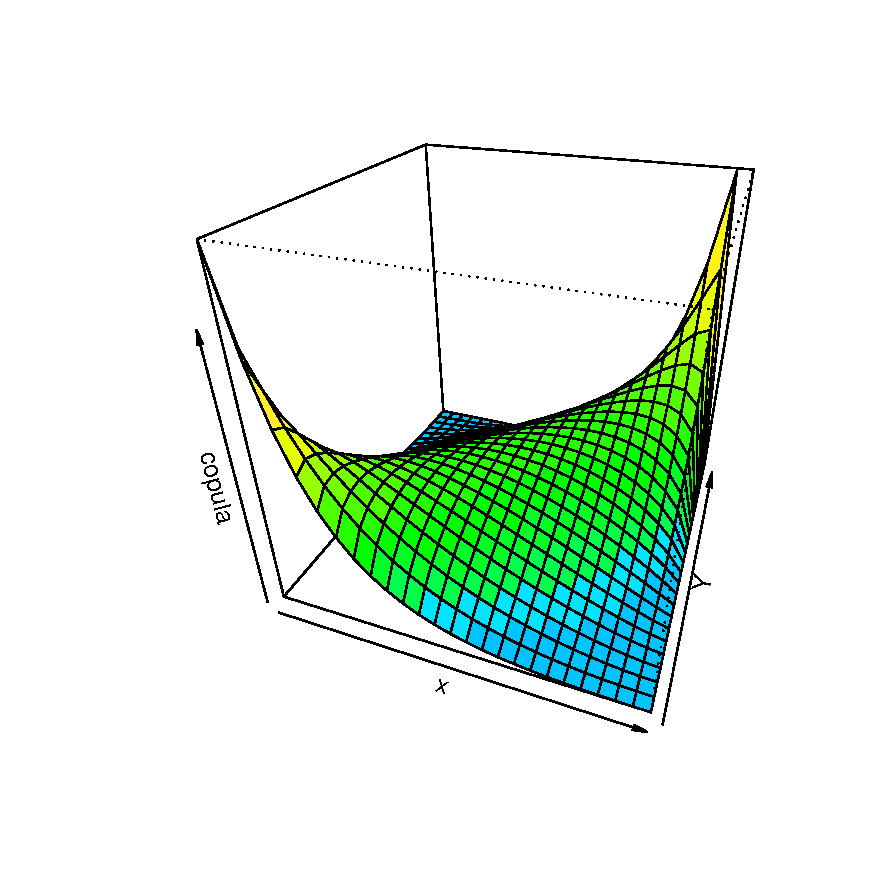
\includegraphics{pictures/Copula.pdf}}}
\caption{\label{fig:copula}A Two-dimensional Gaussian copula}
\end{figure}

This is known as Sklar's theorem \index{Sklar's Theorem} where $C$ is the distribution function of $F$ which shows that the dependence structure can be completely characterised by copula function $C$. This can easily be applied to the default probabilities of obligors within CDOs. Copula functions are extensively described in \cite{nel2005,Sch2003}. There are many copula functions many of which provide better fits for CDO pricing than the Gaussian copula. \cite{hw2004} presents the Double-t and \cite{Sch2003} surveys other copulae which provide alternative default dependence structures.

\subsection{First to default instruments}
\index{FTDs}
\index{First to default}

A First to Default (FTD) basket swap extends CDSs to cover the credit risk for a portfolio of reference entities.  The protection buyer pays a periodic fee of $s$ to the protection seller until either default or maturity of the FTD is reached.  The FTD is terminated after the first default event of any of the reference entities and default payment is then 1-R of the defaulted entity. A typical FTD basket may contain between 4 and 12 reference entities. If the probability of multiple defaults is low then the basket should be well protected by an FTD \cite{Sch2003}. 

FTDs are useful instruments to each side of the FTD contract.  The buyer of protection is able to protect a whole basket of entities at a cheaper cost than purchasing individual default protection and the seller has limited his exposure to one default, his premium for this has increased and the only downside is that the risk of a default payment has increased.
As the size of the basket increases protection given by an FTD weakens and so { \em First Loss Structures } are commonly used.  We do not consider these further though they are detailed in \cite{Sch2003}.

\subsection{$N^{th}$ to default instruments}\label{subsec:NTDs}
\index{NTDs}
\index{N to default}

An $N^{th}$ to default basket swap only differs from an FTD in the specification of the default event, this now being the $n^{th}$ and not the first default event. The valuation of an NTD is based on the probability that the $n^{th}$ default will occur between $T_1$ and $T_2$ as opposed to a standard CDS whose valuation is simply based on default occurring between $T_1$ and $T_2$.  When the $n^{th}$ default occurs the seller pays the notional times $1-R$ and the buyer must pay any accrued payment required to cover the elapsed time since the previous payment.  If we consider a basket of we require application of a Poisson process to generate default probabilities.


\begin{definition}[Poisson Process]\label{def:poisson}\index{Poisson Process}
\begin{rm}
A Poisson process with intensity $\lambda > 0$ is a non-decreasing integer value process with initial value $N(0) = 0$ with independent increments that satisfy, for all $0 \geq t \leq T$
\[
	P[N(T) - N(t) = n] = \frac{1}{n!} (T-t)^n \lambda^n e^{-(T-t)\lambda}
\] 
such that $P(0,T) = e^{-\lambda T}$.  Poisson processes are commonly used within jump diffusion models.
\end{rm}
\end{definition}

The default probabilities within a basket of $n$ entities are generated by Poisson processes with a constant default intensity $\lambda_i$ where $1 \geq i \leq n$, such that
\[
	PS_i(t) = e^{-\lambda T} \quad \mbox{and} \quad PD_i(t) = 1 - e^{-\lambda T}
\]
where $PD_i(t)$ is the risk neutral probability that entity $i$ will default before time $t$ \cite{hw2004}.


Basket Default Swap pricing generally utilises Monte Carlo simulation techniques though in Section~\ref{sec:ntd_surface} we chose to implement the approach presented in \cite{hw2004};
this is a simple process which requires the probability distribution of the number of defaults by a time $T$. This paper also derives a recurrence relationship for the fast computation of this which we implement. \cite{cg2008} present an importance-sampling technique which forces all paths to produce at least $n$ defaults in pricing an
NTD; this increases the probability that the next asset defaults prior to maturity until
$n$ defaults have occurred and requires adjusting the distribution of risk factors to provide more relevent scenarios.\\

The risk neutral pricing of an NTD (where expectations are taken under risk neutral measures) is computed by equating the expected value of the discounted premium payment leg with the expected value of the discounted default leg. In the following, following \cite{Gal03}, $k$ is the seniority of the NTD, $\Delta$ is the time interval between premiums,  $B(0,t_i)$ is the risk free discount factor over interval $(0,t_i)$ and $M$ is the notional. For the premium leg:
\begin{eqnarray}\label{ntd_pl}
 PL & = & E \left[ \sum_{i=1}^n s M \Delta B(0,t_i) 1_{\{\tau_k \leq t\}} \right] \nonumber\\
 & =	& \sum_{i=1}^n s M \Delta B(0,t_i) 1 - F_{k} (t_i) \quad\mbox{where}\quad F_{k} (t_i) = P(\tau_k \leq t)
\end{eqnarray}

and the default leg (DL) is the default premium (DP) less the accrued premium (AP) where
\begin{eqnarray}\label{ntd_dp}
 DP & = &  E \left[M \sum_{i=1}^n (1-R_k) B(0,t_i) 1_{(\tau_k \leq t)} \right] \nonumber\\
 & = &	M \sum_{i=1}^n (1-R_k) \int^T_0 B(0,t_i) F_k dt
\end{eqnarray} 
and
\begin{eqnarray}\label{ntd_ap}
 AP & = & E \left[M \left( s \frac{T_k - t_{i-1}}{t_i - t_{i-1}}  \Delta \right) B(0,\tau_k) 1_{\{t_{i-1} < \tau_k \leq t_i\}} \right] \nonumber\\
&  = & s M \sum_{i=1}^n \int^t_{t-1} \frac{u - t_{i-1}}{t_i - t_{i-1}} \Delta B(0,u) F_k du
\end{eqnarray} 

We can now price the NTD such that s is the fair spread which ensures that PL - DL = 0 to get

\begin{align}\label{ntd_ap}
 s = \frac{ \sum_{i=1}^n (1-R_k) \int_0^T B(0,t_i) F^{kth = j}_k (dt)   }{\sum_{i=1}^n \Delta B(0,t_i) 1 - F_{k} (t_i) + \int^t_{t-1} \frac{u - t_{i-1}}{t_i - t_{i-1}} \Delta B(0,u) F_k du}
\end{align} 

Further detail on pricing NTDs is presented within \cite{Sch2003,Gal03}.

\subsection{Collateralized Debt Obligations}

Collateralized Debt Obligations (CDOs) can be either cash CDOs which consist of credits, debts or loans or synthetic CDOs which can be a portfolio of CDSs. In Figure~\ref{fig:cdostructure} we see an overview of the structure of a CDO instrument. Pricing for CDOs has been widely analysed in \cite{Neu2007,LBG2008}. As with other derivative instruments a CDO consists of fixed and floating legs, $X_F$ and $X_V$, respectively where you receive $X_F$ and pay $X_V$ and the premium is chosen such that $X_F = X_V$.

CDOs are divided into a tranche structure $[K_L,K_U]$ where $K_L$ is the attachment point and $K_U$ is the detachment point. Each tranche is fixed such that the NPV of cashflows paid is zero. Holders of tranche $[K_L,K_U]$ have limited their loss exposure to $K_U - K_L \% $ of the initial portfolio value. Losses are paid by tranche holders during the life of a CDO with a predetermined frequency.  Holders of a tranche $j$ with $[K_L,K_U]$  receive periodic payment with frequency $\nu$, usually 0.25 years, equal to a premium $s_j$ of the outstanding notional of the tranche. Loss $L_{t,j} = min (L_t,K_U) - min (L_t,K_L)$ is a percentage of total portfolio loss.  The structure of cash flows for tranche $j$ holders at each payment date receive $X_F$ and pay $X_V$ where
$ X_F = s_j \nu \Gamma_{j,t} $ and 
$	X_V = (Z_{j,t}-Z_{j,t-\nu})M  $ for $t = \nu, 2\nu, \ldots, T$ and $s_j$ fixed and $\Gamma_{j,t}$ is the outstanding notional, a decreasing function of portfolio losses and total portfolio loss is $L_t M$.   The outstanding notional is given by
\begin{align}
\Gamma_{j,t} = \begin{cases} 
						(K_U-K_L)M & L_t < K_L \nonumber \\
						(K_U-L_t)M & K_L \leq L_t \leq K_U  \\
						0			& L_t \geq K_U 
				\end{cases}
\end{align}


In these products the originator may retain the equity tranche to show that the issuing bank knows best the riskiness of the credits and that it holds the riskiest tranche is a clear signal that this is a fair deal to enter into.


\begin{figure}
\centerline{\scalebox{0.8}{\includegraphics[viewport = 107 510 497 786]{pictures/CDOStructure.pdf}}}
\caption{\label{fig:cdostructure}The Structure of a CDO}
\end{figure}


\subsection{LHP One Factor Gaussian Copula CDO Pricing}

Assumptions of the Large Homogenous Portfolio (LHP) \cite{lp2007} are:
\begin{enumerate}
\item The reference portfolio is homogenous so all assets share the same pairwise correlation, default probabilities and recovery rates.
\item The number of assets in the portfolio tends to infinity.
\item The default dependency structure is based on a Gaussian Copula model.
\item Each tranche is priced on a single flat correlation, the compound correlation of the tranche.
\end{enumerate}

Default of each obligor is condtionally independent given a level of state risk $M$ and occurs if  $X_i = \sqrt{ \rho } M + \sqrt{ 1 - \rho } \epsilon_i$ is less that a threshold where $M$ and $\epsilon_i$ are independent normal variables.

The LHP Gaussian Copula models the default correlation using a firm value approach.  We begin by modeling the default dependency structure assuming all assets are correlated with a single market variable, following the formulation of \cite{Sch2003}:
\begin{align}\label{eq:onefactor}
X_j(T) = \sqrt(\rho) Z + \sqrt(1-\rho) \epsilon_j		\quad	\forall_j = 1, 2, \ldots, n
\end{align}
where $cov(\epsilon_i, \epsilon_j) = 0$ for $i \neq j$ and $cov(Z,\epsilon_i) = 0$ for all $i$.
$\rho$ is the correlation of asset values with the market factor M. $\epsilon_j$ is the idiosyncratic firm specific risk.  This process is similar to the CAPM (Capital Asset Pricing Model) formulation of splitting risk into two components.  As we assume that M and all $\epsilon_j$'s are normal this is the gaussian copula model.

$X_j(T)$ is the value of a firm $j$'s assets at time $T$. When $X_j(T)< K(T)$ where
$K(T)$ is our default barrier the firm experiences default.  Applying~\eqref{eq:onefactor} into this and rearranging for idiosyncratic risk gives us:
\begin{align}\label{eq:epFactor}
\epsilon_j \leq \frac{K(T) - \sqrt(\rho)M}{\sqrt(1-\rho)}
\end{align}

Now we seek the probability of default conditional on $M$:
\begin{eqnarray}
 p_j(t,T \mid M) & = & Prob[X_j(T)< K(T)\mid M] \nonumber\\
 & = & Prob[\epsilon_j \leq \frac{K(T) - \sqrt(\rho)M}{\sqrt(1-\rho)} \mid M ]  \nonumber\\ 
 & = & \phi \left( \frac{K(T) - \sqrt(\rho)M}{\sqrt(1-\rho)} \right) \nonumber \\
& = & \phi \left( \frac{\Phi^{-1}(1 - e^{-s(T-t)}) - \sqrt(\rho)M}{\sqrt(1-\rho)} \right)
\end{eqnarray}

We can now apply the important large portfolio assumption and assume that the number of defaulted credits is provided by the individual default probabilities conditional on $M$.  The loss fraction makes use of the recovery rate
\begin{align}
l_{pf}(t,T \mid M) = (1-R)  p_j(t,T \mid M)
\end{align}
and from this we can derive the payoff of a particular tranche condtional on $M$.  The unconditional loss, where the integral removes the dependency on $M$, is:
\begin{align}
EL^b_a(t,T_i,\rho ,s,R) = \int^\infty_{-\infty} Payoff\left[ a,b,l_{pf}(t,T \mid M) \right] \psi(M) dM \nonumber \\
= \int_{-\infty}^\infty \frac{1}{b-a}\left[ (l_{pf}(t,T \mid M)-a,0)^+ - (l_{pf}(t,T \mid M)-b,0)^+ \right] \psi(M) dM
\end{align}

This can be solved with numerical integration.  Losses start to erode the capital on a tranche only when all subordinate tranches are wiped out. \cite{HPW2005} show that correlation is positively dependent on default probabilities.




\subsection{Valuing a CDO swap}\index{CDO! Swap}

The price of a CDO swap is given by the following expression (further detail in \cite{Eli2006}):
%%\begin{equation}
\begin{eqnarray}
 V_{CDO}(0) & =  & E\left(\int^{T}_{0} \mathrm{e}^{- \int^t_0 r(u) du } dL_{[K_L,K_U]} (t) \right) \nonumber\\ 
& & - c E\left(\sum^{Q}_{i = 1} \mathrm{e}^{- \int^t_0 r(u) du } \delta_i \frac{(N_{[K_L,K_U]}(T_i) + N_{[K_L,K_U]}(T_{i-1}))}{2}  \right) \nonumber\\  
 & = & E\left(\int^{T}_{0} \mathrm{e}^{- \int^t_0 r(u) du } dL_{[K_L,K_U]} (t) \right) - c A_{[K_L,K_U]}(0)
\end{eqnarray}

where $A_{[K_L,K_U]}$ is the price of a risky annuity. Hence the breakeven spread, the coupon $c$ value which
ensures that the fixed and floating legs have the same value, is:

\begin{align}\label{credSpread}
 c_{BE}(0) = \frac{E\left(\int^{T}_{0} \mathrm{e}^{- \int^t_0 r(u) du } dL_{[K_L,K_U]} (t) \right) }{ A_{[K_L,K_U]}(0)}
\end{align}



%%\end{equation}

\subsection{Monte Carlo CDO Pricing}\index{CDO! Pricing}

Much work on pricing CDOs uses Monte Carlo simulations as any forward-rate based model has a very large state space.  An unbiased estimator will be generated to approximate the {\em true} price of a CDO.  As each trial is independent we can apply the central limit theorem which tells us that our difference between the true value and the simulation value is normally distributed with zero mean so we can approximate the sample standard deviation and from this we can form confidence intervals. More trials can be conducted it we then want to increase the simulation accuracy.  Monte Carlo processes are fully examined in \cite{Sch2003}.
\cite{hw2004} also present a useful methodology for pricing CDOs without Monte Carlo simulation.

\subsubsection{Multi-factor models}

The random variables defined in equation~\ref{eq:onefactor} can be extended to many factors with the following change
\begin{align}\label{eq:multifactor}
V_j(T) = \sqrt(\rho_1) M_1 + \ldots + \sqrt(\rho_n) M_n + \sqrt(1-\rho_1 - \ldots - \rho_n ) \epsilon_j			\forall_j = 1, 2, \ldots, n
\end{align}
such that the $M_i$ have independent distributions with zero mean and unit variance.  An example of the requirement for such a model might be within a global portfolio where there are stong intra-country correlations or if there are sector links within a portfolio. This models are covered within \cite{hw2004,Schm2003}.


\subsubsection{Student-t Copula Functions}

The Gaussian Copula one factor model is still considered the industry standard for CDO pricing \cite{Eli2006} but many other alternatives have been considered including the Double-t Copula \cite{hw2004} and the normal inverse gaussian \cite{Neu2007}, the latter of which we do not consider further.  The Double-t Copula essentially replaces the Gaussian one-factor model with one that is t-distributed on both systematic and idiosyncratic risk. The t-distribution should increase the more extreme values for the assets and so increase the probability of observing more defaults.


\subsection{Success of CDOs}\index{CDO! Success of}

The iTraxx and CDX indices of CDS on 125
names can themselves be structured and traded like a traditional synthetic CDO with
equity, mezzanine, and senior tranches. Like in a traditional CDO, the
standard tranches of CDS indices provide claims to the cash flows of the iTraxx CDS
portfolio, in return for payments by the investors if a default occurs within their tranche. 

CDOs have been immensely successful in the marketplace for many reasons including potential for spread arbitrage opportunities, the transfer of risk and, as noted in \cite{Gib2004}, that tranche sensitivities can be linked in to the business cycle.


\subsection{Single Tranche Trading}\index{CDO! Single Tranche Trading}

iTraxx tranches (or the iTraxx index itself) can also be used by
arrangers for the dynamic hedging of single-tranche CDOs. Single tranche traders have historically focussed on the mezzanine tranche so they may be riskier as they are unlikely to be fully hedged.

\subsection{Random Recovery Rates and Random Factor Loading}

\cite{as2005,Neu2007} present extensions to the form factor model shown in equation~\eqref{eq:onefactor} based on random factor loading. An example is the two point loading of \cite{as2005} where $X_j(T) = a_{ij}(Z) Z + v_j \epsilon_j + m_i$ 
\begin{align}
a_{ij} \left(Z_j \right) =  \begin{cases} 
						\alpha_{ij} & Z_j \leq \theta_{ij} \nonumber\\
						\beta_{ij} & Z_j > \theta_{ij}  
					 \end{cases}
\end{align}
and $\alpha_{ij},\beta_{ij}$ are positive constants and $\theta_{ij} \in \mathbb{R} $.  This can be viewed as a switching model where loading takes values $\alpha_{ij}$ with probability $\phi(\theta_{ij})$ and  $\beta_{ij}$ with probability $1-\phi(\theta_{ij})$ so if $\alpha_{ij} > \beta_{ij}$ then the factor loadings will decrease in $Z_j$. As the random factor model changes the correlation through factor exposure as a function of the factor itself this could represent asset values coupling more strongly to a poor economy.

\medskip
Despite the standard models assuming a standard recovery of 40\% research has shown these actually vary with credit event (i.e. default,rating up/downgrades). \cite{as2005} allow recovery rates to have both an idiosyncratic and a systematic risk factor.  Recovery rates are specified as $R = \phi(\mu_i + \gamma_i V + \sigma_{\epsilon_i} \epsilon_i)$. \cite{kre2008} extends this letting the recovery rate have a default triggering factor. In this model each obligor has a discrete recovery distribution noting that the average recovery rate must equal the quoted recovery rate so that consistency with the single name CDS market is maintained.  This model applies in scenarios where standard base correlation fails such as when spreads widened in March 2008 and senior tranches could not be priced. \cite{AH2008} present a similar extension.


\section{Implied Correlation}\index{CDO! Implied Correlation}\index{Implied Correlation}

The Black-Scholes model for pricing options presents a formula where the option price is a function of rate, time to maturity, underlying stock price and stock price volatility. When we have a market price of the option we can infer the volatility. This is the {\em implied volatility }. With the advent of the credit indices we can infer the default correlation coefficient from the given market spread.  Increasing maturities of CDOs will also lead to the generation of a forward correlation curve.


\begin{definition}[Volatility Smile]
\begin{rm}
The pattern that at-the-money options have a lower volatility than other options. The volatility smile will generally be calculated for vanila options and will then be used for more complex option modeling.
\end{rm}
\end{definition}

\subsection{The Implied Correlation Curve and the Credit Indices}

Given the market price of a single tranche CDO, the Vasicek Single Factor model and the default correlation coefficient $\rho$ we can compute $\rho$ which matches the price of a CDO.  For each tranche we can compute the implied default correlation.  This presents us with the problem of the { \em correlation smile }, where the spread for mezzanine tranches is lower than that of the equity and senior tranches.  Mezzanine tranche premiums are non-monotonic which unfortunately provides us with non-unique tranche premiums. If the pricing mechanism of equation~\eqref{credSpread} were correct there would be no { \em correlation smile}. We present a generated smile for iTraxx data for 31 July 2008 in figure~\ref{fig:impCorr}.

\begin{figure}
\centerline{\scalebox{0.5}{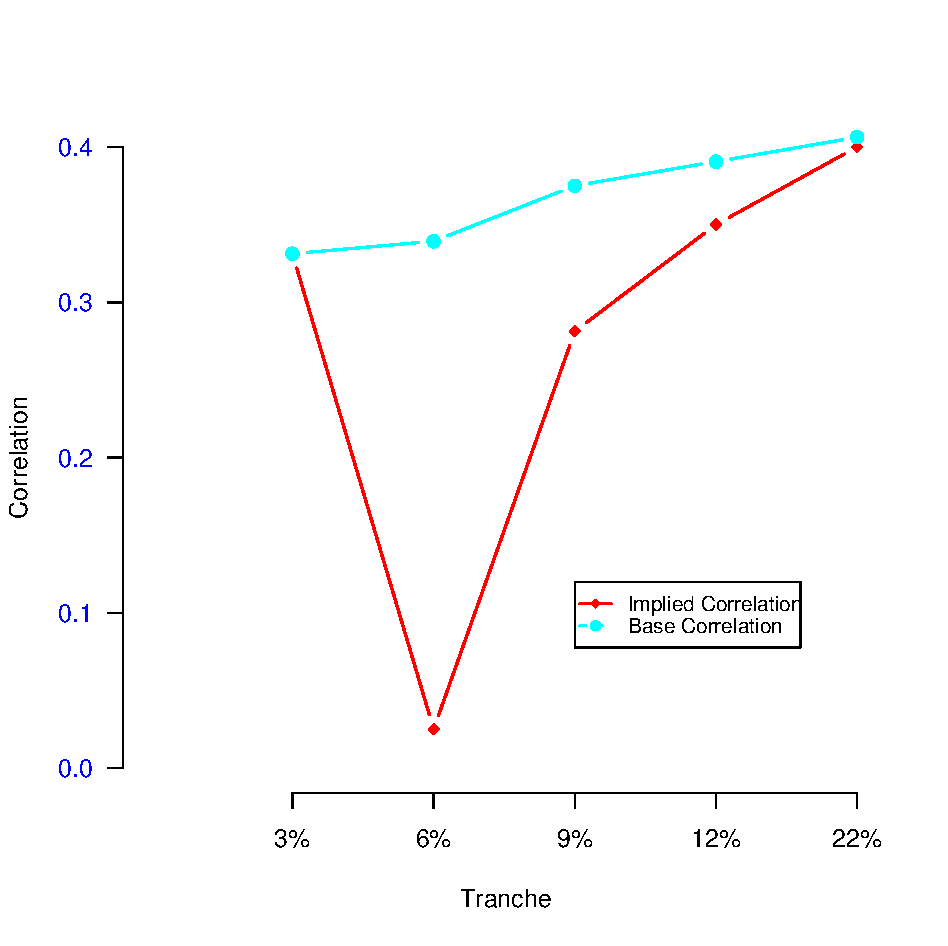
\includegraphics{pictures/impliedCorr.pdf}}}
\caption{\label{fig:impCorr}iTraxx EU S9 Implied and Base Correlation for 31 July 2008}
\end{figure}

Reasons for the correlation smile, collated in \cite{Eli2006}, include:
\begin{enumerate}
\item Different investor groups purchase different tranches and, hence, may have different views on correlations
\item Unknowns in correlation models affecting equity tranches, which are more sensitive to correlations, which may contain a model risk premium embedded in their prices
\item Variations in local demand conditions in prices
\item Disparities between different pricing models
\end{enumerate}

The implied correlation issue is still a contentious area within credit risk.  As noted in \cite{risk2006}, implied volatility can be assessed historically but it is far more difficult to view historical time to default correlations.

\subsection{Base Correlation Pricing Mechanisms}

Base correlation, introduced by \cite{MA2004}, uses the guaranted monotonicity of the equity tranche and proceeds to construct fictitious equity tranches which are used to construct mezzanine and subsequently senior tranches. This recursive { \em bootstrapping } technique relies on applying the implied correlation from the previous tranche.

Base correlation replaces implied correlation on the standard tranches with virtual tranches which all have the same lower attachment point of 0\%. So the set of virtual tranches contains $0 - K_U\%$ where the detachment point in $K_U \in { 3,6,9,12,22 }$. Any tranche can then have its loss decomposed into two tranches which have a $0\%$ detachment point to give us:-
\begin{align}
E(L[0,K_j])=E(L[0,K_{j-1}]) + E(L[K_{j-1},K_{j}])
\end{align}

Base Correlation allows for non-standard tranches to be easily priced and interpolated.
\cite{pw2007} show that extrapolation can be dangerous outside this and lead to arbitrage opportunities. 

Base Correlation is generated using the following bootstrapping process \cite{KL2004}:-
\begin{enumerate}
\item	Find the Equity Tranche Implied Correlation as for the standard compound correlation process. This requires solving for $0 = PV(0,K_1,S_{0,K_1},\rho_{K_1})$	
\item	For the next tranche we solve for $0 = PV(0,K_2,S_{K_0,K_1},\rho_{K_2}) - PV(0,K_1,S_{K_1,K_2},\rho_{K_1})$.  Note that the second term here uses $\rho_{K_1}$ from the previous step so we still have one equation with one unknown.	
\item	Iteratively apply step 2 to higher tranches.
\end{enumerate}

Base Correlation produces a correlation skew as shown in figure~\ref{fig:impCorr}. Each tranche is base correlation pricing is considered an equity tranche which is long correlation so all tranche PVs are increasing functions of the upper attachment point.
There is much debate as to whether base correlation is a suitable model or simply a process to remove the correlation smile. \cite{risk2006} notes that it is not arbitrage free, does not consider invidual spreads and all credits are equally weighted. In Spring 2008 the index spreads for senior tranches widened and base correlation methods failed \cite{kre2008}\footnote{and personal experience within Credit Risk IT!}. \cite{KL2004} presented scenarios where this would occur when the junior mezzanine tranche spreads were high which is what occurred in 2008 as these high spreads inverted the initial curve making it impossible to price senior tranches.





\chapter{Price Surface Investigation Results}\label{chap:study}


\section{Parameter Calibration}\label{sec:param_cal}\index{Parameter Calibration}

Parameter calibration for multi-name credit derivative pricing focuses on three areas:
\begin{enumerate}
\item Generation of the default probabilities within models (or the use of external rating agency information).
\item Loss Given Defaults (and recovery rates) which are necessarily different if the CDO is cash or synthetic.
\item The default correlation whose modeling is considered a difficult problem in CDOs \cite{Gib2004}. Equity correlation as a model for default correlation is insufficient.  What is the precise relationship between equity returns and default correlation?  They are probably not the same.
\end{enumerate}

We conduct simulations for NTDs and CDOs looking a varying recovery rates and correlations.  Additionally we look at varying intensities in NTDs and default probabilities with varying factor sensitivities in CDOs.

\section{NTD Pricing Surfaces}\label{sec:ntd_surface}

In figure~\ref{fig:BasketSpreads} we see the spreads of an NTD (seniority=6) increasing in correlation but falling with respect to recovery rate. Spreads increase with correlation and, for fixed correlation, increase with intensity as recovery rates decrease (figure~\ref{fig:BasketSpreads},right).  Clearly many defaults should occur in periods of high intensity and when recovery rates are low spreads should increase.

\begin{figure}
{\scalebox{0.5}{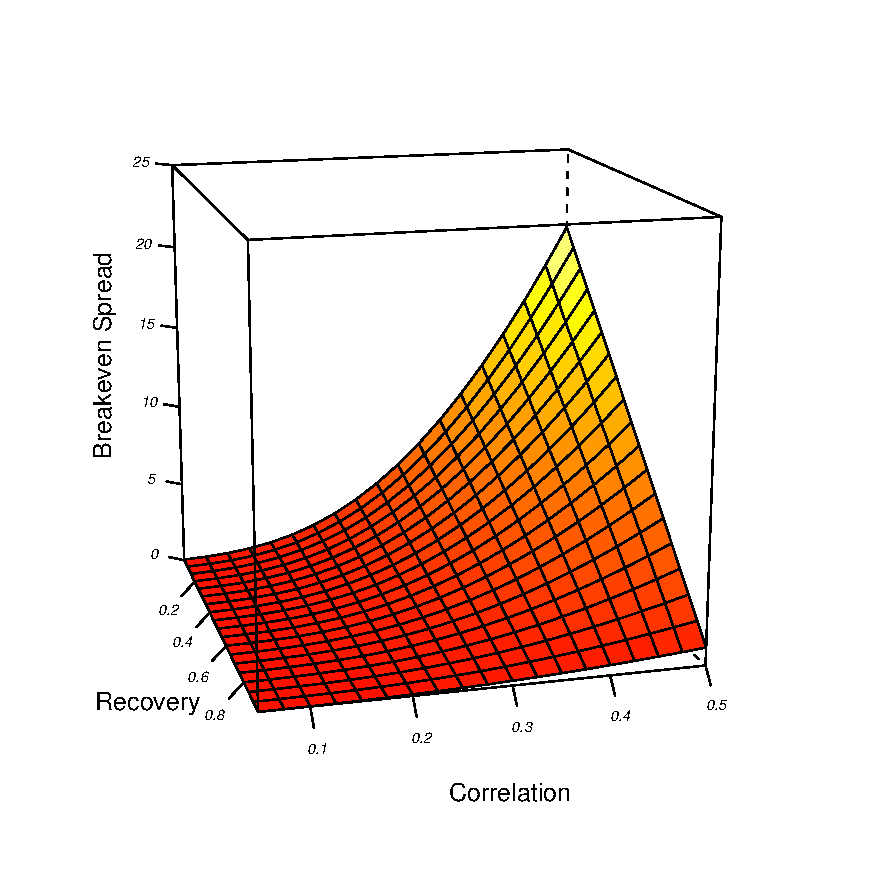
\includegraphics{pictures/BasketSpreads_Aug24.pdf}}}
{\scalebox{0.5}{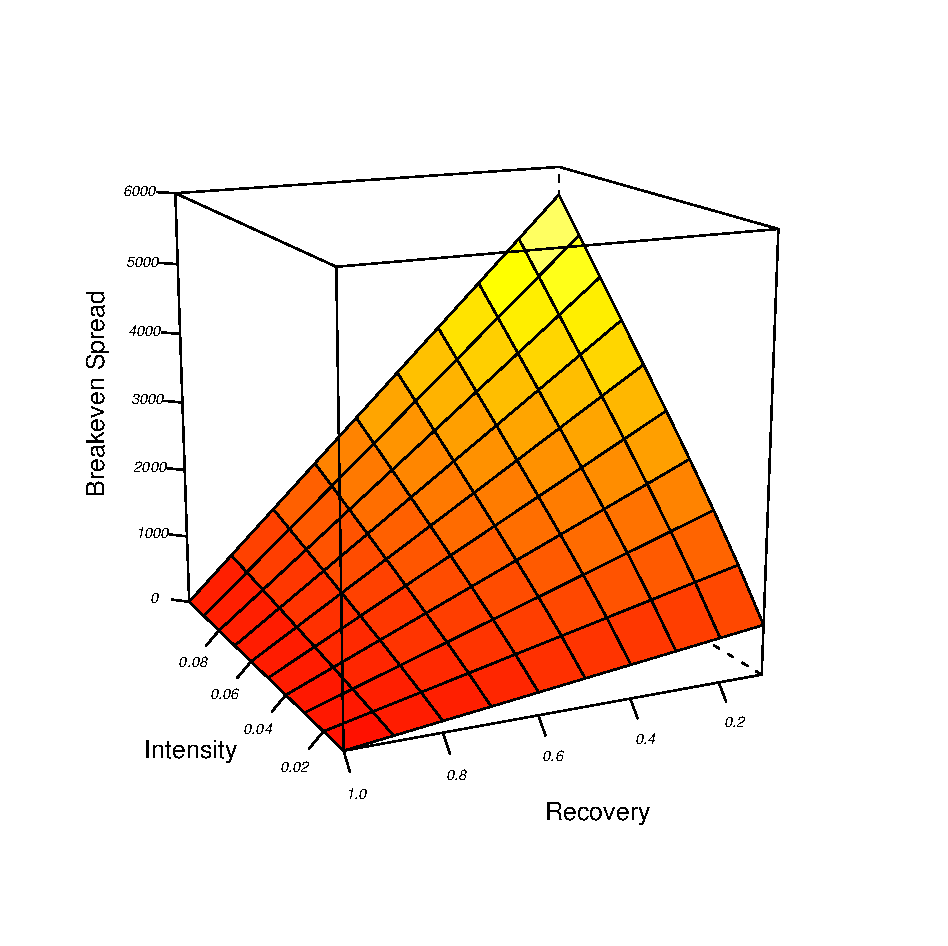
\includegraphics{pictures/BasketSpreadsIntensityRec_Aug27.pdf}}}
\caption{\label{fig:BasketSpreads}NTD Spreads for a basket of 10 entities considering the 6th to default with varying recovery rate, intensity and correlation}
\end{figure}

\begin{figure}
{\scalebox{0.5}{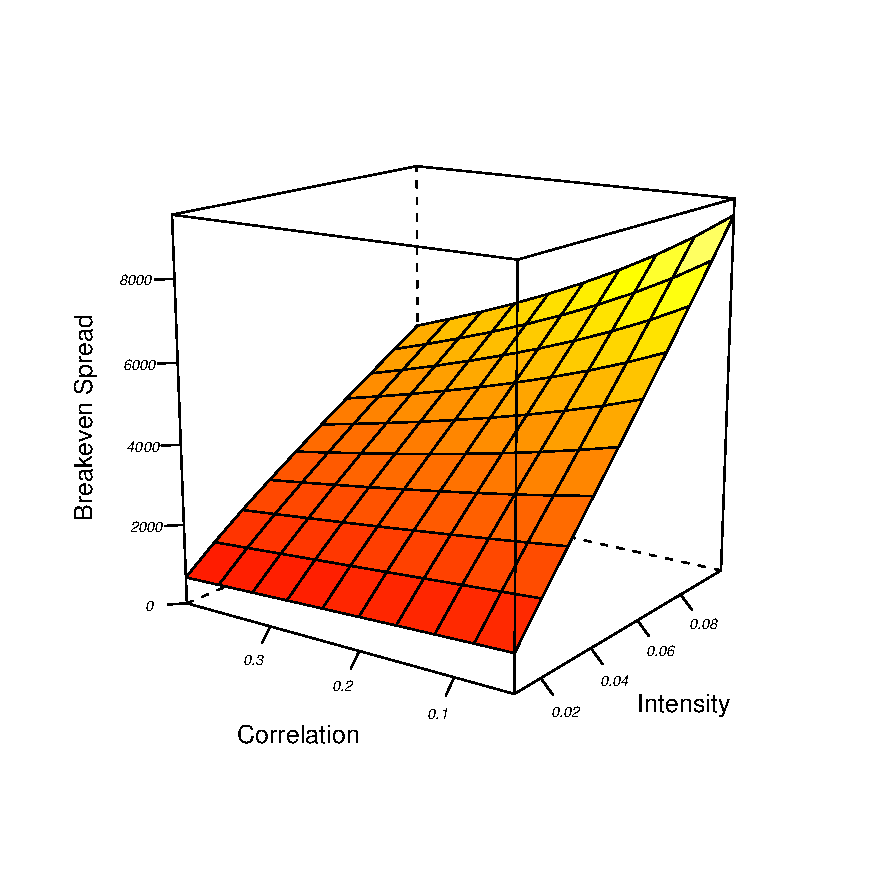
\includegraphics{pictures/BasketSpreadsFTDIntensity_Aug25.pdf}}}
{\scalebox{0.5}{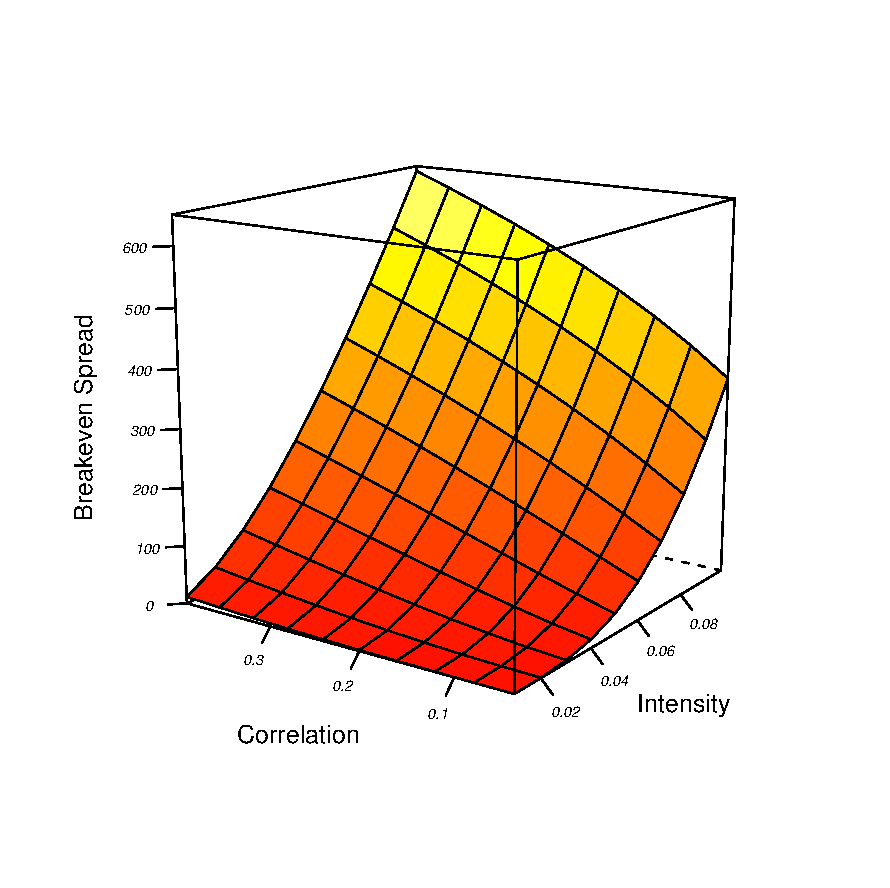
\includegraphics{pictures/BasketSpreadsIntensity_Aug24.pdf}}}
\caption{\label{fig:IntensityBasketSpreads}A comparison of intensity for a basket of 10 entities considering the 1st to default (left) and the 6th to default (right) with varying correlation and default intensity}
\end{figure}


\subsection{The effects of default intensity}

In figure~\ref{fig:IntensityBasketSpreads} we compare the intensity of a First to default (NTD, seniority = 1) against that of a 6th to default basket swap with varying correlation.  As the correlation increases we see the spreads increase for the higher default $n$ in an NTD whilst decreasing for the FTD.  Why is this so?  If our basket were perfectly correlated defaults would occur simultaneously and so the NTD spreads would be the same for all $n$.  For a much lower correlation, close to 0, the spreads decrease as it is highly unlikely for the defaults to cluster.  This becomes more pronounced as the default intensity itself increases, as we can see. The rate of increase is decreasing for low $n$ (figure~\ref{fig:IntensityBasketSpreads},left) and increasing for higher $n$ (figure~\ref{fig:IntensityBasketSpreads},right). This result extends Table 1 of \cite{hw2004} which shows this for 3 intensity points.  For very low intensities we see that increasing correlation lowers the spreads very slightly for FTDs and raises them for NTDs.  As intensities themselves increase correlation becomes more important so the correct intensity must be chosen within basket swap modeling. \cite{hw2004} looks at the dispersion of intensities relative to an average of 0.01 and finds that convexity is increased raising the prospect of one default and lowering the prospect of multiple defaults.


\section{CDO simulations}\label{sec:cdo_exp}

\subsection{Gaussian vs. Student-t Copula}\index{Copula Functions! Comparision}

Firstly, we present our spreads achieved for CDO pricing and compare a normal against a student-t distribution. \cite{Eli2006} states that the normal gaussian cannot fit prices of different CDO tranches with a single $\rho$ though the Student-t copula corrects this but does require more computation. In Figure~\ref{fig:tranchespreads} we compare spreads computed using Gaussian and Student-t distributions with 4 degrees of freedom. We see that across correlations the Student-t distribution is slightly higher for the equity tranche and slightly lower for the remaining tranches. A Student-t distribution should allow for more extreme events and so we should see more defaults in the equity tranche and fewer in the senior tranches, accounting for these differences.  Note that this spread structure of figure~\ref{fig:tranchespreads}, using our R CDO Pricing routine (see~\ref{sec:cdo_price}), is in line with published results \cite{hw2004,bv2005}. Variation of the degress of freedom of the $t$-distribution would be another avenue for interesting results.


\begin{figure}
{\scalebox{0.45}{\includegraphics{pictures/TrancheSpreads.pdf}}}
{\scalebox{0.45}{\includegraphics{pictures/TrancheSpreads_studentt.pdf}}}
\caption{\label{fig:tranchespreads}Tranche Spreads across Correlations for Equity, Mezzanine and Senior Tranches of a CDO}
\end{figure}

We examine the exposure to correlation risk \cite{Gib2004} wherein it is noted that tranches have sensitivity to the business cycle given that tranches have a dependency on default correlation and this may therefore be considered to be a business cycle risk.  \cite{Gib2004} refers to this as "most insightful".

\begin{figure}
{\scalebox{0.5}{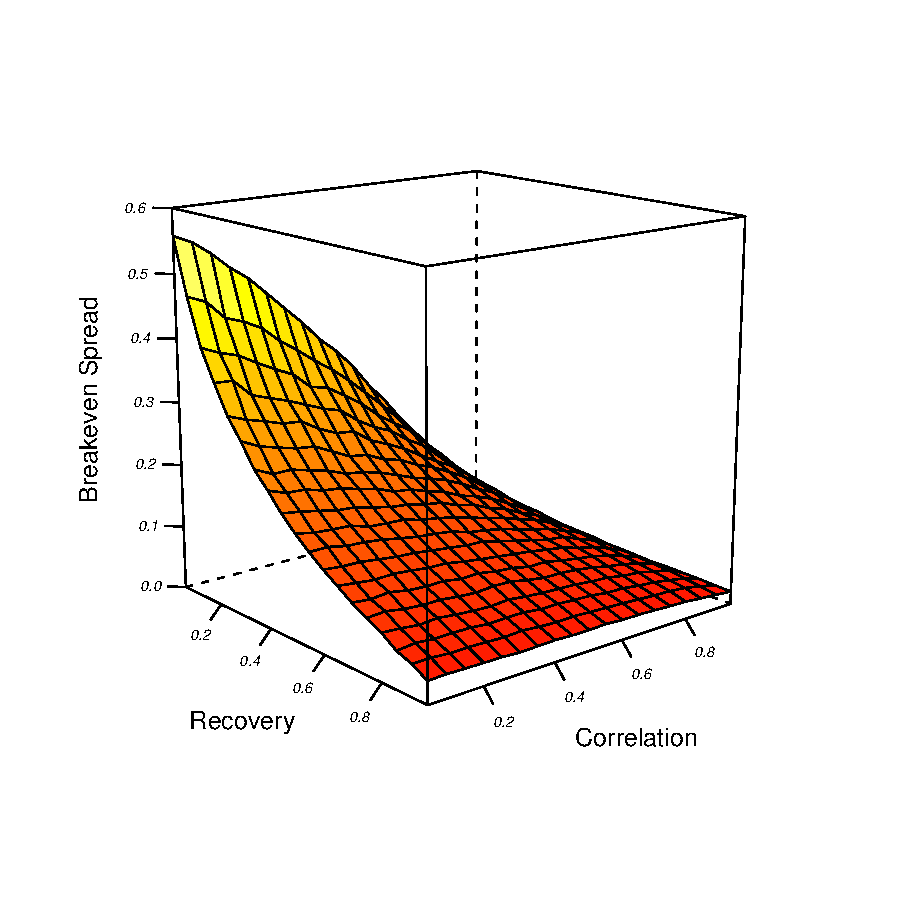
\includegraphics{pictures/CDOsim_June30_RecCor_EqTranche.pdf}}}
{\scalebox{0.5}{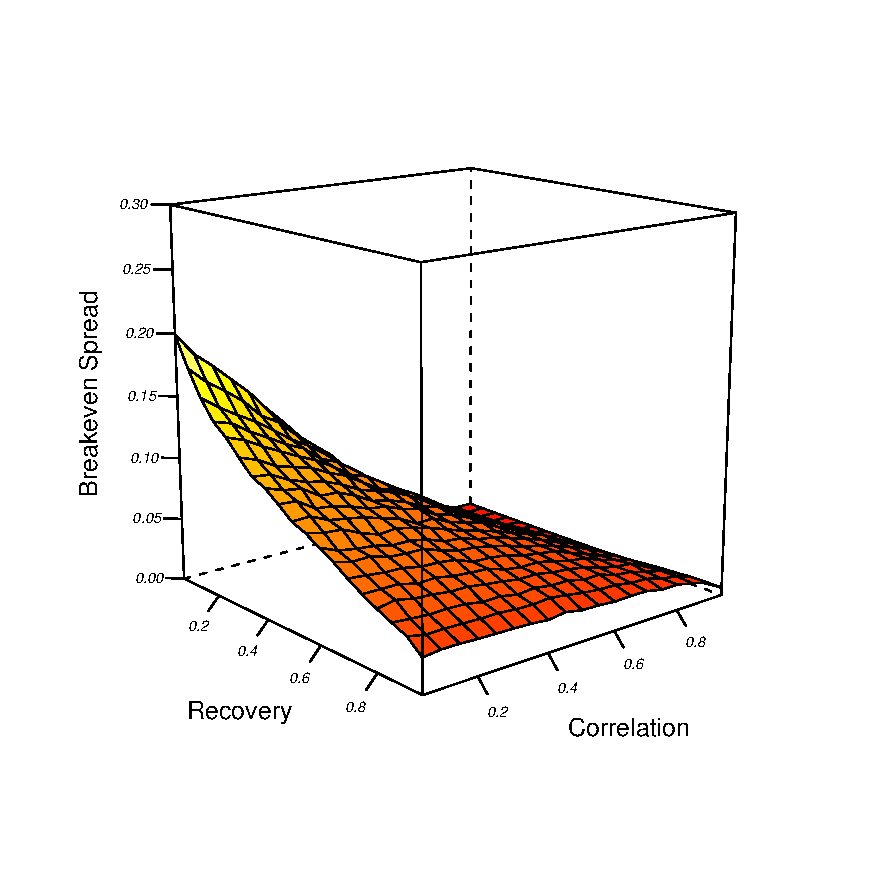
\includegraphics{pictures/CDOsim_Aug18_RecCor_MezzTranche.pdf}}}
{\scalebox{0.5}{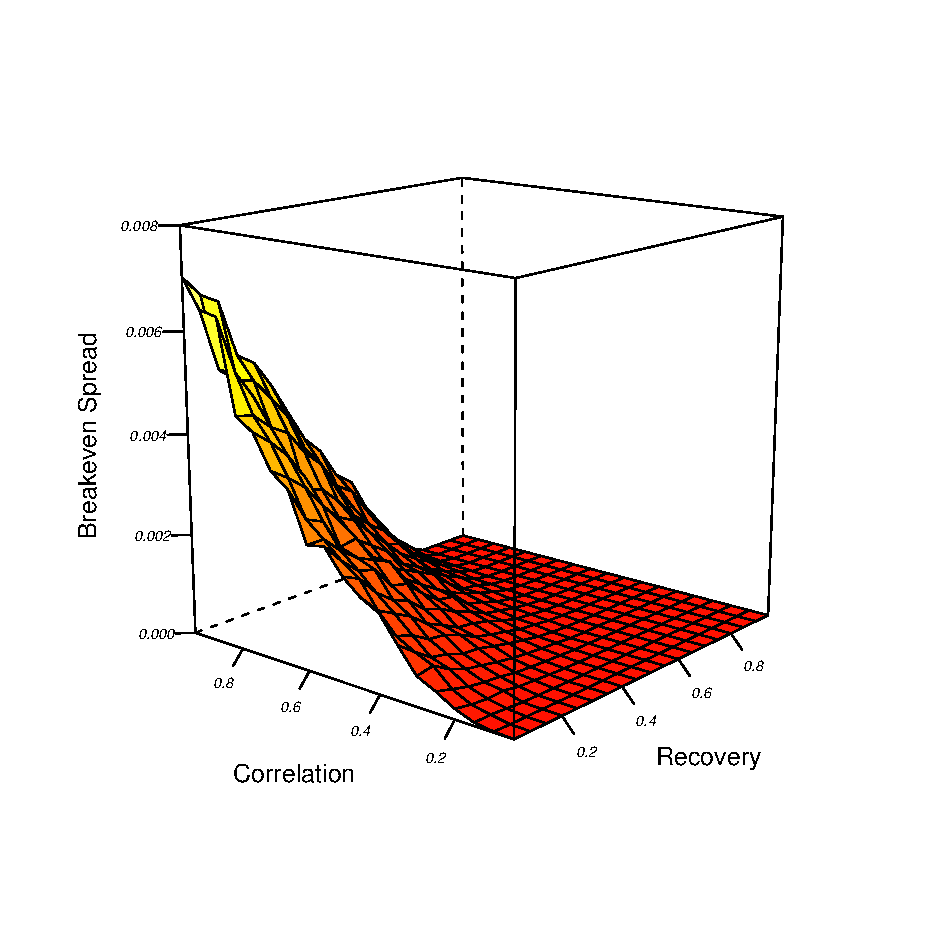
\includegraphics{pictures/CDOsim_Aug28_RecCor_SupSenTranche22_100.pdf}}}
\caption{\label{fig:CorRecSurface}Equity, Mezzanine and Senior Tranche for CDO, simulations varying recovery rate and correlation (Spreads:bps)}
\end{figure}

\subsection{Tranche Comparison}

In figure~\ref{fig:CorRecSurface} we present simulations for the equity (0-3\%, top left), mezzanine (6-9\%, top right) and super senior tranche (12-22\%, bottom) of a CDO generating the breakeven spread across recovery rates and correlation defaults. Mezzanine spreads are lower that those of the Equity tranche with the Senior  and Super Senior tranches being even lower.

 We see that the the higher correlation the higher the default probabilities and a decrease in premium which is monotonic on default correlation.  Clearly for the senior tranche the breakeven spreads are much lower but we can still see that the higher the recovery rate and the lower the correlation the higher the spread. Junior Mezzanine (3-6\%) and senior (9-12\%) tranches exhibited the same behaviour as mezzanine and super senior tranches but with slightly higher and lower, respectively, spreads. Figure~\ref{fig:CorRecSurface} shows that the correlation spread relationship for equity and mezzanine tranches is inverted for senior tranches. In the figure we highlight a super senior tranche (bottom) of 12-22\% which exhibits the same surface as a senior tranche but with lower spreads.  Why do we see this inversion across tranches? The reason for this is that the senior tranche is only likely to experience default when there are multiple defaults (high correlation) and the equity tranche (first loss tranche) is affected by any defaults. Even then we have seen that the spreads are small and any correlation must be high for the senior tranches.

We also see a slight saddle from high correlation / low recovery rate to high recovery rate/ low correlation in Equity and Mezzanine tranches, the effect being more pronounced in the latter. This is most probably due to the mezzanine tranches affected by second/third losses.

\begin{figure}
\centerline{\scalebox{0.5}{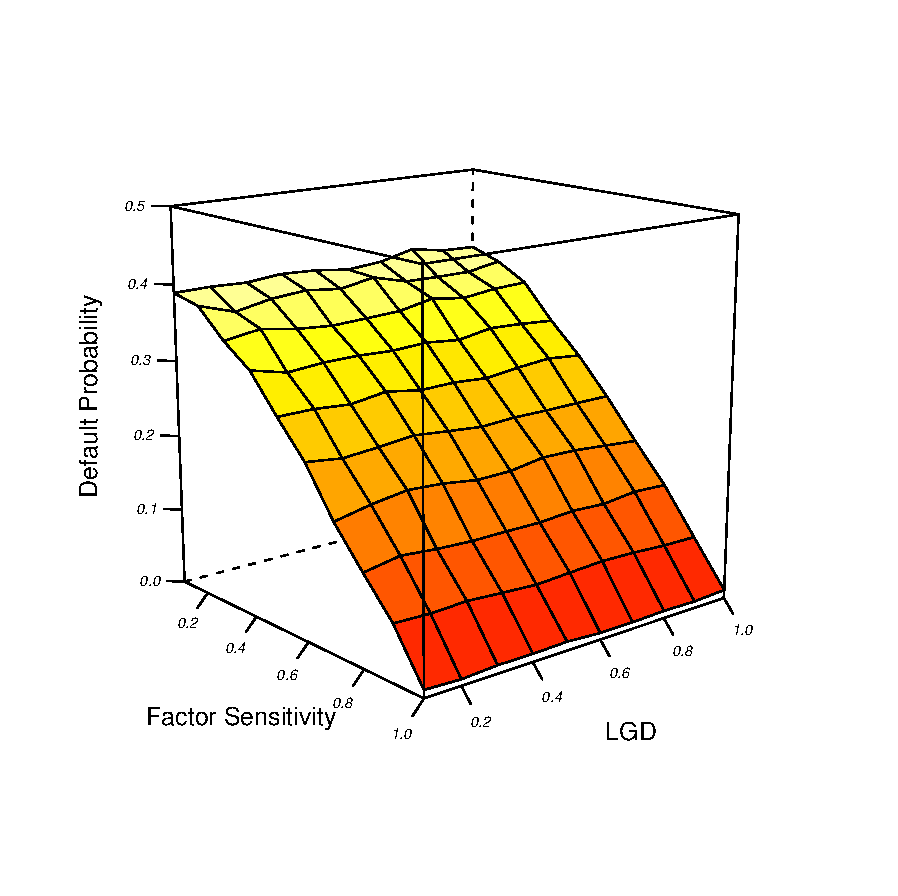
\includegraphics{pictures/EqTranche.pdf}}}
\centerline{\scalebox{0.5}{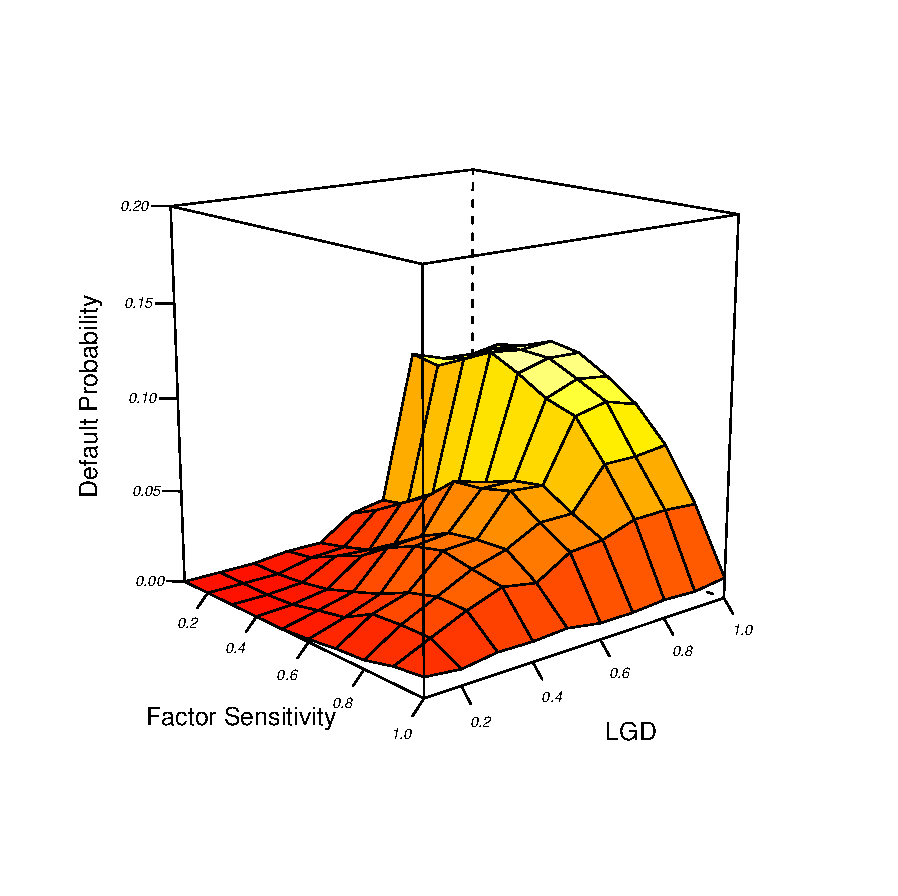
\includegraphics{pictures/MezzTranche.pdf}}}
\centerline{\scalebox{0.5}{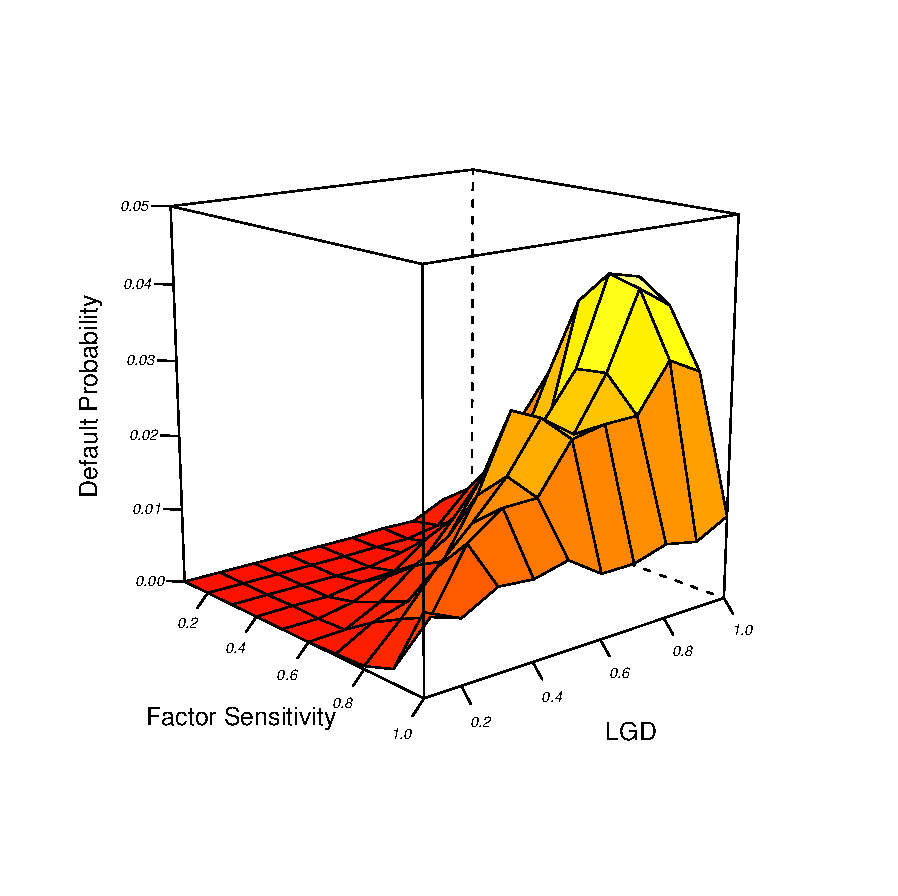
\includegraphics{pictures/SenTranche.pdf}}}
\caption{\label{fig:Unknown copula density}Equity,Mezzanine and Senior Tranche across LGDs and Factor Sensitivities (Spreads:bps)}
\end{figure}

\subsection{Factor Sensitivity}

In Figure~\ref{fig:Unknown copula density} we show results for simulations of a portfolio of 50 assets running 10000 simulations for each point. For the equity tranche we see the probability of default decrease as the factor sensitivity increase for all possible LGDs. This factor sensitivity to systemic risk suggests that the economy is {\em good} and so default probability will be low. Any increases in factor sensitivity (correlation) suggest there is more chance of no default occurring. As the LGD increases the default probability increases sharply around 0.7 but at a decreasing rate for increasing factor sensitivity.

 In the mezzanine tranche the probability of default increases slowly then decreases as LGDs increase and for the senior tranche the probability of default sharply increases then sharply decreases in increasing LDGs.  Factor sensitivity and LGD must be high for there to be a non-negligible default probability within the senior tranches. High correlation within the senior tranche implies that there is a chance of multiple defaults and we see this for figure~\ref{fig:Unknown copula density} (bottom).  The generation of these default probabilities replicates how ratings agencies use default probabilities to assign ratings to CDO tranches.




\section{Base Correlation - Why use this?}\index{Base Correlation}


In Figure~\ref{fig:tranchespreads} we see that for the Mezzanine and Sub-Senior tranches there are two correlations for a particular spread.  This means that standard implied correlation generates two solutions and motivates the requirement for base correlation. A Base Correlation skew is shown in figure~\ref{fig:impCorr}.
We note that data obtained for this work for the CDX and iTraxx indices shows that spreads have significantly increased since the publication of \cite{KL2004,hw2004}.



\chapter{Summary and Conclusion}\label{chap:conclusion}

In this report we have introduced Credit Derivative Pricing mechanisms. 
Additionally we have investigated price surfaces for these products.

The Credit Crisis of 2007 resulted in even the senior tranches having their ratings
downgraded.  Effects of this were exemplified in citigroup losing \$43 billion on its
books despite most of this being held within CDO senior tranches \cite{econ2008cracks}.


\section{Credit Derivatives and Basel II}\label{sec:conc_baselII}\index{Basel II}

Under Basel I for every dollar lent to a corporation it was required that the lending bank held 8 cents in equity, irrespective of its ratings whether it was AAA or CCC.  Basel II was formulated to introduce a sensitivity to the risk of exposure.

For Banks, high exposure to CDO equity tranches will generate high capital charges under Basel II.  Basel II show that the correlation coefficient is a function of the default probability. The Basel Committee employ a one-factor model of portfolio credit risk \cite{lp2007}. Basel II will align regulatory capital charges with actual credit risks. This will provide more recognition of hedged portfolios \cite{Gib2007}. In the light of the Credit Crisis early application of Basel II might have reduced the losses incurred by the large banks.  As we have stated banks held most of the equity tranches and our simulations, in line with market data, have shown this to be the most costly tranche.

\section{Tranching and the Credit Crisis of 2007}\label{sec:conc_crisis}\index{Credit Crisis}

Credit Derivative instruments are based upon bilateral contracts whose pay out is linked to the performance of a credit claim issued by a third party.  As such they have 3 characteristics which, I believe, have led to their success in the past few years.  Firstly, they enable clear separation between the creditor and the risk-bearer. Secondly, the claim, if made, will be on the contract counterparty not on the third party issuing the contract.  Finally, and of most import in the subprime crisis, they allow for the structured selling of credit risk positions including the shorting of credit.  This repackaging of loans, interest payments, and other default risks into securities has allowed more people to gain access to credit.  It is this securitisation of the subprime sector which caused the current crisis.  Many of the CDOs counted on volatility remaining low and used high leverage instruments; these were the first instruments to see losses. As the notional amount of outstanding credit derivatives began to exceed the actual amount of underlying debt credit exposure was leveraged through these credit derivatives. This incentivised the reason to create credit risk \cite{fgz2004} leading to an overall increase in systematic risk within the system, which we saw develop in mid 2007.\\

What were the triggers? Was it the end of the teaser rates and the first defaults on the part of subprime borrowers occurring in late Spring 2007?  In June 2007 Moodys downgraded 131 Asset Backed Securities (ABS) and 5 days later Bear Stearns announced that 2 of their hedge funds had suffered losses on subprime securities and were close to being shut down.  One hedge fund received a \$3.2 billion bail out but further deals were downgraded in July 2007 by both Moodys and S\&P including 184 CDO tranches.  As a result of this banks suddenly became reluctant to lend to each other; the overnight libor rates shot up as any counterparty could now be a bad risk.  By August 2007 some funds were frozen citing an inability to value them under the current market conditions. It was time for the central banks to step in.
The structuring of the credit instruments meant that they could be marked 3A1 by ratings agencies as lenders split the products from their risk of default.  This was obviously a miscalculation on their part and should never have happened.  Can we now trust the ratings agencies given that they are paid by the firms which created these credit securities?  In their defence they have correctly stated that their job was to measure credit and not liquidity risk. The question of whether a AAA rated corporate bond should be treated the same as a AAA senior tranche of a CDO remains open. 

\medskip
In Spring 2008 spreads of senior tranches had widened to such a degree that the Gaussian Copula model no longer worked.  Industry {\em quick} fixes to this of lowering recovery rates, or as suggested in \cite{Kre2008,AH2008}, of using random recovery rates seem to have rapidly been applied.

It is also important to note that credit derivatives do not eliminate credit risk but merely shift it around. The recent crisis has suggested that many market participants did not fully consider their credit riskiness when entering into CDO positions. As stated in \cite{bv2005} the top 15 global banks held three quarters of all credit risk protection that had been bought or sold; this was surely a cliff edge on which to stand.


\section{Directions for future research within Credit Derivatives}


This report notes the following {\em important} open problems:
\begin{itemize}
\item Valuing a CDO$^2$ - There is no real way to know the correct correlation for these so are Gaussian Copulas in any way the correct function to use? 
\item Exchange traded futures based on iTraxx indices to be launched.  This will increase the liquidity and transparency of Credit Derivative products.
\item Applying computationally intensive optimisation processes to derive the correlation structure of CDOs from tranche spreads. There are numerous optimization methodologies for achieving this and we refer the interested reader to \cite{hs2006} who make use of Evolutionary Algorithms.
\item Incorporating multifactor pricing models would have provided an interesting avenue for further work within this project.
\item Further study of random recovery rates and random factor loadings, particularly in the current market.
\end{itemize}

\section{Conclusions}

Credit Derivatives are an immature market \cite{Gib2007} but their huge increase in growth over the last decade shows how eager firms are to manage and transfer their credit risk.  After the initial fluctuations of the credit crisis it is highly likely that complex credit products will become even more popular though with more caution from all investors.

In this project we have provided an overview of the Credit Derivatives market, defined and motivated CDOs and NTDs (including FTDs). We have examined the pricing of these instruments as their determinant parameters are varied, such as the recovery rate, correlation, default intensity and factor sensitivity.  These simulations were implemented in $R$, their structure is defined in Appendix~\ref{app:sim_meth} and, for completists, the code itself is in Appendix~\ref{app:code}.  We have also used the pricing mechanisms of CDOs to study the implied correlation {\em smile} and the base correlation {\em skew}.  We have presented a (brief) comparison of these pricing models. We have concluded that there are difficulties with the base correlation model in the light of current market conditions and this is currently a rapidly developing area.

\medskip

Our conclusions are as follows:-
\begin{enumerate}
\item	We have shown that NTD spreads vary with the default position and this is a downward slope for increasing correlation for lower seniority NTDs (e.g. FTD where seniority = 1) and an upward slope for higher seniorities.  A higher correlation suggests less chance of default for FTD and more for NTDs. Intensity was also examined and can lead to sharp increases as it varies (figure~\ref{fig:IntensityBasketSpreads}).
\item	We have shown that CDO tranche spreads vary according to the tranche and differently with correlation between tranches. High equity tranche spreads are generated by the Gaussian copula pricing approach and these suffered the greatest losses in the Credit Crisis of 2007-2008.
\item We have examined factor sensitivities and default probabilities and shown that these have an inverse relationship between the equity and the mezzanine/senior tranches. Factor sensitivities need to be high for senior tranche default.
\item The correlation smile was found for recent market data and so we implemented a base correlation approach. Interesting avenues exist for developing this further including random recovery rates and random factor loadings and if the market problems of 2008 with base correlation pricing are not to occur again further work must be carried out.
\end{enumerate}






{\setlength{\baselineskip}{14pt}
\bibliography{CredDeriv}
}

\appendix

\chapter{Simulation Methodology}\label{app:sim_meth}

We now describe our process for conducting simulations.  The code was implemented in is S language and executed within the R system.  
Additional R packages were used for implementation purposes. \cite{yan2007} presents an interesting overview of the R copula package.

\section{Simulation Details: Pricing Credit Derivatives}\label{sec:sim_er}

\subsection{Simulation Implementation Decisions}

To generate a matrix of correlated standard normal variables $X = (X_1, X_2, \ldots, X_n)$ we can either:
\begin{enumerate}
\item Apply a Cholesky decomposition\footnote{A symmetric positive-definite matrix can be efficiently decomposed into a lower triangular matrix $L$ and $L^T$} to $\Sigma = AA^T$, generate $n$ i.i.d. standard normal random numbers $z_1, z_2, \ldots z_n \in N(0,1)$ and set $\underline{X} = A\underline{z}$ where
$X = (X_1, X_2, \ldots, X_n)$ are correlated random numbers fitting the joint normal distribution, or
\item Apply the form factor model shown in equation~\ref{eq:onefactor}
\end{enumerate}

In our code shown in Appendix~\ref{app:code} we show NTDs implemented with the latter and CDOs implemented via application of Cholesky decomposition.

\medskip

\subsection{Verification of Code}\label{subsec:code_verif}

Results for our pricing code were initially verified using equivalent input data to that of \cite{hw2004,KL2004}.  We then proceeded to conduct our simulations on more recent data obtained from {\em datastream} and http://www.creditfixings.com.\\

Tables 1 and 2 were used for comparing NTDs and Tables 7 to 9 were used for verification of our CDO pricing process.  Default probability were also compared with sample data provided in \cite{lp2007} within spreadsheet format.



\subsection{Solving for Implied and Base Correlation}\label{subsec:impCorrSolve}

Our implied and base correlation figures were achieved using a simple one-dimensional
root solving procedure.  This is provided in $R$ with the uniroot function and extensions
of this.  We reimplemented this to achieve bespoke functionality for CDOs using a simple
bisection process.

\subsection{Monte Carlo Procedures}\label{subsec:monte}

We outline the procedure for a Monte Carlo generation of the default leg of 
an NTD \cite{Sch2003}.

\begin{enumerate}
\item Generate independent samples of standard normal variables $Z_0, Z_1, \ldots , Z_n$
\item Generate correlated normal variables with $X_i = \sqrt{ \rho } M + \sqrt{ 1 - \rho } \epsilon_i$, $1 \leq i \leq n$.
\item Set $U_i = \phi(X_i)$, $1 \leq i \leq n$ and $\tau_i = F_i^{-1} (U_i)$, $1 \leq i \leq n$
\item Set t to the $n^{th}$ order statistic of $t_0, t_1, \ldots , t_n$
\item Set the discounted payoff = $(1 - R) * I(\tau \leq T) * P(0, \tau)$
\item Repeat step 1 to 6 m times to obtain the confidence interval of the default leg. This can then be constructed with the m copies of the discounted payoff.
\end{enumerate}

For accuracy we set $m = 50000$ or $m = 100000$.
\smallskip

\subsection{Accuracy of Monte Carlo Simulations}\label{subsec:accuracy}

Monte Carlo processes can take many hours to run and do not guarantee a correct result.  How do we assess what simulation size we will have an accurate result within tolerance limits?

We could do the following:
\begin{enumerate}
\item	Run our desired simulation for a very large number of trials (from 1-10 million)
\item	Run for a specific number of trials that can be easily repeated (say 50000 ). This provides us with an unbiased estimator to the true value.
\item	Assess our sample statistics and standard error comparing stages 1 and 2 and form a confidence interval for our price (based on the central limit theorem).  If stage 2 presents us with a confidence interval that is still too large then we increment out sample size by, say, 10000, and return to stage 2.  Repeat this until we are inside our tolerance levels.
\end{enumerate}

Time constraints for this project prevented a more formal analysis of our choice of simulation size for NTD and CDO pricing.



\chapter{Code Listings}\label{app:code}

This appendix contains the R source code developed for this project. 
Base Correlation required simple extensions to the standard CDO pricing method
and the implied correlation method whereby the price of the previous equity tranche
is incorporated into the current price, given that this is fixed. This is fully detailed in \cite{KL2004} and not
presented to save space.

\section{CDO Pricing}\label{sec:cdo_price}
\begin{singlespace}
\lstset{basicstyle=\scriptsize, 
keywordstyle=\color{black}\bfseries,
commentstyle=\color{white}, % white comments
stringstyle=\ttfamily, % typewriter type for strings
belowskip=0pt,
aboveskip=0pt,
showstringspaces=false}

\begin{lstlisting}
# function created for matrix generation
repmat <- function(a,n,m) {kronecker(matrix(1,n,m),a)}

CDOPrice <- function(N,R,lambdaf,rho,n,c,a,d,r,No,flag)  
{  
 # N - number of entities
 # R = recovery rate
 #lambdaf = default intensity
 #rho = pairwise correlation
 #n = 1
 #c = 1
 #a = attachment point in \%
 #d = detachment point in \%
 #r = risk free rate
 #No = Number of simulations
 #flag = 1

 TM <- 5                     # length of the CDO     
 tstep <- 0.5                # the coupon payments     
 nn  = n * N                 # the total notional     
 loss = n * ( 1 - R)         # the total loss where R is recovery Rate
 T <- seq(0,TM,tstep)        # vector for the fixed coupon dates     
 Tmod <- t(array(rep(T,N), dim=c(length(T),N))) # matrix of fixed coupon dates for all N companies     
 discount <- exp(-r*T[2:length(T)])   # discounted fixed coupon vect

# just to initialize the generator     

 MRho = repmat(rho,N,N);      # initialize the correlation matrix     
 for (i in 1:length(MRho[1,])) { MRho[i,i] <- 1 }  # fill diagonal entries with 1      
     
 MRho <- chol(MRho)          # doing the Cholesky factorization     
 fixedtot <- 0                # initializing for fixed leg total     
 floattot <- 0                # initializing for floating leg total     
 sqfixtot <- 0                # for standard error estimate     
 sqfltot  <- 0                # for standard error estimate   

 Values <- N * No
 PMat <- array(rnorm(Values),dim=c(N,No)) # N rows, No columns
  
 PMat1 <- t(MRho) %*% PMat         # to get the correlated Gaussian matrix  
   
 PMat11 <- pnorm(PMat1) # take the CDF to make them a copula     

 PMat2 <- -log(1 - PMat11)/ lambdaf    # inverse function to get the default time    

# Begin MC simulations 
 for (i in 1:No)                   # loop for different paths of MC 
{       
 PMat3 <- PMat2[,i]                # getting the i'th path        
 Pmatmod <-repmat(PMat3,1,2*TM+1)  # getting it for the fixed coupon dates        
 Temp1 <- Pmatmod < Tmod           # keeping default times that are only within the CDS maturity        
 Lmat <- loss*Temp1                # getting the losses matrix * defaults            
 Tloss <- colSums(Lmat)            # sum  losses         
 Ploss <- Tloss/nn                 # get loss percentages  
 PlossSum <- rep(0,length(Tloss))
 for (j in 1:length(Ploss))
	{ PlossSum[j] <- max(Ploss[j]-a,0) - max(Ploss[j]-d,0)        }
 #Plossum <- max(Ploss-a,0)-max(Ploss-d,0)  # getting the loss percentage in the tranche         
 Lossum <- PlossSum*nn                        # getting the absolute loss in the tranche         
 tempplos <- PlossSum[2:length(PlossSum)]-PlossSum[1:length(PlossSum)-1] #          
 temp2 <- nn * tempplos         
 temp <- nn*(d-a-PlossSum)                        # getting the notional left in the tranche                
 coupon <- tstep*(temp[1:length(temp)-1] + temp[2:length(temp)])/2 # getting the fixed coupons 
        
 fl_flows <- discount*temp2                      # getting the discounted floating flows         
 fx_flows <- discount*coupon*c                  # getting the discounted fixed flows         

 Vfloat <- sum(fl_flows)                          # the total floating flows for this path         
 floattot <- floattot + Vfloat                  # the total floating flows until now         
 sqfltot  <- sqfltot  + (Vfloat^2)              # to get the standard error square term         
 Vfixed <- sum(fx_flows)                          # the total fixed flows for this path         
 fixedtot <- fixedtot + Vfixed                  # the total fixed flows until now         
 sqfixtot <- sqfixtot + (Vfixed^2)              # to get the standard error square term     

}    

# End MC simulations



result <- 0
result[1] <- fixedtot/No    
#Monte Carlo floating leg estimate  
result[2] <- floattot/No    
#CDO Value estimate   
result[3] <- (floattot - fixedtot)/No    
#Monte Carlo Breakeven Spread 
result[4] <- floattot/(fixedtot/c)    
#Monte Carlo Fixed leg std error
result[5] <-  (1/No) * sqrt(sqfixtot - ((1/No) * (fixedtot^2)))    
#Monte Carlo Floating leg std error 
result[6] <- (1/No) * sqrt(sqfltot - ((1/No) * (floattot^2)))     

# return the breakeven spread ALONE for simulation purposes
return(result[4])

}

\end{lstlisting}
\end{singlespace}

\section{NTD Pricing}

\begin{singlespace}
\lstset{basicstyle=\scriptsize, 
keywordstyle=\color{black}\bfseries,
commentstyle=\color{white}, % white comments
stringstyle=\ttfamily, % typewriter type for strings
belowskip=0pt,
aboveskip=0pt,
showstringspaces=false}
\begin{lstlisting}

#Calculates spread of nth to default swap using procedure mentioned  
#in Appendix A of Hull and White 2004 paper 
#Valuation of an Without Monte Carlo Simulati NTD
# using a recurrence relationship.

#getBasketSpread(0.01,10,1,0.3,0.4,5)
#getBasketSpread(0.01,10,2,0.3,0.4,5)
#getBasketSpread(0.01,10,3,0.3,0.4,5)
#getBasketSpread(0.01,10,4,0.3,0.4,5)
#getBasketSpread(0.01,10,5,0.3,0.4,5)

getBasketSpread <- function(intensity,obligors,seniority,corr,rec,maturity)
{

#--------- Parameters  ---------- 
lambda<-intensity  	#Default intensity for all firms 
N<-obligors  		#No of obligors 
k<-seniority  		#seniority level eg 2nd to default swap 
rho<-corr  			#correlation between each pair of entities 
T <- maturity  		#maturity of default swap 
r<-0.05  			#risk free rate  
Recovery_rate<-rec  	#recovery rate 
delta <- 0.5  		#semi-annual fixing 
ntimesubsteps<-4  	#no. of sub timesubsteps within each delta for int 
#---------------------------------------   


bdebug<-0  
n<-T/delta  #time steps for indexing preminum payments 
dt<-delta  
dt2<-dt/ntimesubsteps   

tmpintegrand <- function(M) 	
{

	ai<-rho^0.5  	
	Qi<-1-exp(-lambda*g_t)	# Follow a Poisson process
	Fi<-qt(Qi,5)  	
	ai2<-(1-ai*ai)^.5  
	#tadjust<-(rchisq(1,5)/5)^0.5
	K <- M *sqrt(0.6)
	#K <- M
	tmp<-(Fi-ai*(K))/ai2  	
	Si<-(1-pt(tmp,5))  	#probability of survival of each firm 	
	piT0<-Si^N  		#probability that all firms will survive 
	wi<-(1-Si)/Si
	 	
	Vvec<-array(c(rep(wi,N)),dim = c(1,N))

	idxvec<-array(c(1:N),dim = c(1,N))
	Vvec<-N*(Vvec^idxvec)  	
	Uvec<-array(c(rep(0,N)),dim = c(1,N))

	Uvec[1]<-Vvec[1]  	
	piTvec<-array(c(rep(0,N)),dim = c(1,N))  	

	for(ki in 2:N)
	{ 		
		tmpsum<-0  		
		for(ki2 in 1:(ki-1)) 	
		{		
			tmpsum <- tmpsum-(-1)^(ki2)*Uvec[ki-ki2]*Vvec[ki2]
		}
	
		tmpsum <- tmpsum+(-1)^(ki+1)*Vvec[ki]	
		Uvec[ki] <- (tmpsum/ki)
	}

	piTvec<-outer(Uvec,piT0,"*")
	
	survival_prob<-1-sum(piTvec[k:N]) 
	
	return(survival_prob*dt(K,5))

}  

if (bdebug == 0)	
{
	SurvivalProbMat<-array(0,dim=c(ntimesubsteps*n+1,2))	
	t1<-0
	for(i in 1:length(SurvivalProbMat[,1]))
	{ 		
		g_t<-t1  		
		SurvivalProbMat[i,1]<-t1 
		result<-integrate(Vectorize(tmpintegrand),-10,10)

		numRes<-as.numeric(result[1])
		SurvivalProbMat[i,2] <- numRes
		t1<-(t1+dt2)  	
	} 
}

#SurvivalProbMat  
DP<-0  #Expected value of average default leg payments 
PL<-0  #Expected value of average Premium leg payments 
AP<-0  #Expected value of average Accrued premium  

for (i in 2:length(SurvivalProbMat[,1]))
{ 	
	t<-SurvivalProbMat[i,1] 	
	B<-exp(-r*t)  	
	defaultProb<-(1-SurvivalProbMat[i,2])-(1-SurvivalProbMat[i-1,2])  	
	DP<-DP+(1-Recovery_rate)*B*defaultProb  
	if ((t%%delta) < 0.01) 		
	{
		PL<-PL+delta*B*SurvivalProbMat[i,2]  		
		AP<-AP+delta*B*defaultProb  			
	}
	else if (t > delta)
	{
		tgap<-t%%delta 		
		AP<-AP+tgap*B*defaultProb  	
	}
}

#DP 
#PL 
#AP  

spread<-10000*DP/(PL+AP)
return(spread)

}

\end{lstlisting}
\end{singlespace}




\section{Implied Compound Curve Generation}\label{sec:imp}

\begin{singlespace}
\lstset{basicstyle=\scriptsize, 
keywordstyle=\color{black}\bfseries,
commentstyle=\color{white}, % white comments
stringstyle=\ttfamily, % typewriter type for strings
belowskip=0pt,
aboveskip=0pt,
showstringspaces=false}
\begin{lstlisting}

implied_correlation <- function(mktSpread, lower, upper, initialCorr=0.3)
{

	ACCURACY <- 1.0e-3
	MAX_ITER <- 100
	HIGH_VALUE <- 1
	ERROR <- -1e40

	corr_low <- 1e-4
	corr_high <- initialCorr
	
	spread <- getSpread(corr_high,lower,upper)


	while (spread < mktSpread)
	{
		corr_high <- 2.0 * corr_high
		spread <- getSpread(corr_high,lower,upper)

		if (corr_high > HIGH_VALUE) return(ERROR)

	}

	for (i in 0:MAX_ITER)
	{
			
		corr <- ((corr_low + corr_high) * 0.5)
		spread <- getSpread(corr,lower,upper)
		test <- spread-mktSpread
		if (abs(test) < ACCURACY)
		{
			return(corr)
		}

		if (test < 0.0) 
		{ 
			corr_low <- corr 
			print('test is less than 0')
		}
		else
		{
		  	corr_high <- corr
			print('test is greater than 0')

		}

	}

	return(ERROR)
}

\end{lstlisting}

\end{singlespace}

\section{Default Probability Generation}

\begin{singlespace}
\lstset{basicstyle=\scriptsize, 
keywordstyle=\color{black}\bfseries,
commentstyle=\color{white}, % white comments
stringstyle=\ttfamily, % typewriter type for strings
belowskip=0pt,
aboveskip=0pt,
showstringspaces=false}
\begin{lstlisting}


Simulations <- 100000
Loans <- 50
Tranches <- 3

w <- 0.3 ## what is this in the Nomura correlation primer doc?

attachmentPoints <- c(0.0,0.03,0.07,1)
EADs <- rep(1,Loans)
LGDs <- rep(0.5,Loans)
defaultProbs <- rep(0.01,Loans)
attachmentPoints
EADs
LGDs
defaultProbs

sumEADs <- sum(EADs)
sumEADs

normalizedEADs <- EADs/sumEADs
normalizedEADs

d <- qnorm(defaultProbs)
d

wArray <- rep(w,Loans)
w2Array <- rep( (1 - w*w)^0.5, Loans)
wArray
w2Array

# rnorm(1,mean=0,sd=1) 
factor <- rnorm(1)
factor

tranchePD <- rep(0,length(attachmentPoints)-1)
currentLoss <- rep(0,Loans)
length(attachmentPoints)

for(i in 1:Simulations) 
{
	factor <- rnorm(1)
	factor
	loss_j <- 0
	for (j in 1:Loans)
	{
		if ((wArray[j] * factor + w2Array[j] * rnorm(1)) < d[j]) 
		loss_j <- (loss_j + (LGDs[j] * normalizedEADs[j]))
	}
  
	for (k in 1:(length(attachmentPoints)-1))
	{
		if (loss_j - attachmentPoints[k] > 10^-15)
		{
			tranchePD[k] = tranchePD[k] + 1/Simulations
		}
	}

}


simCDO <- function(matri,c1,c2,Sims,PortfolioSize)
{

lgd=matri[c1];
w=matri[c2];

Simulations <- Sims
Loans <- PortfolioSize
Tranches <- 3
attachmentPoints <- c(0.0,0.03,0.07,1)
EADs <- rep(1,Loans)
LGDs <- rep(lgd,Loans)
defaultProbs <- rep(0.01,Loans)

sumEADs <- sum(EADs)
normalizedEADs <- EADs/sumEADs
d <- qnorm(defaultProbs)
wArray <- rep(w,Loans)
w2Array <- rep( (1 - w*w)^0.5, Loans)
factor <- rnorm(1)

tranchePD <- rep(0,length(attachmentPoints)-1)

for(i in 1:Simulations) 
{
	factor <- rnorm(1)
	factor
	loss_j <- 0
	for (j in 1:Loans)
	{
		if ((wArray[j] * factor + w2Array[j] * rnorm(1)) < d[j]) 
		loss_j <- (loss_j + (LGDs[j] * normalizedEADs[j]))
	}
  
	for (k in 1:(length(attachmentPoints)-1))
	{
		if (loss_j - attachmentPoints[k] > 10^-15)
		{
			tranchePD[k] = tranchePD[k] + 1/Simulations
		}
	}

}

	return(c(tranchePD))

}

\end{lstlisting}
\end{singlespace}


\section{Example of a surface generation in R}\label{sec:surface}
\begin{singlespace}
\lstset{basicstyle=\scriptsize, 
keywordstyle=\color{black}\bfseries,
commentstyle=\color{white}, % white comments
stringstyle=\ttfamily, % typewriter type for strings
belowskip=0pt,
aboveskip=0pt,
showstringspaces=false}
\begin{lstlisting}

simCDO2 <- function(matri,c1,c2,sims,trancheLow,trancheHigh)
{
rec=matri[c1];
correl=matri[c2];
	return(c((CDOPrice(100,rec,0.01,correl,1,1,
				trancheLow,trancheHigh,0.04,sims,1))))

}
recovery <- seq(0.05,0.95,by=0.05)
correlation <- seq(0.05,0.95,by=0.05)
t1 <- rep(recovery,19)
s1 <- rep(correlation,each=19)

m1 <- cbind(t1,s1)

spreads <- apply(m1,1, simCDO2, c1="t1", c2="s1", 
				trancheLow=0.06, trancheHigh=0.09, sims=10000)


trellis.par.set("axis.line", list(col="transparent"),
	clip = list(panel = "off"))

trellis.par.set(theme = col.whitebg())
poly.border<-trellis.par.get("box.rectangle")
poly.border\$border<-"green"
trellis.par.set("box.rectangle",poly.border)

fig5 <- wireframe(spreads ~ t1 * s1, 
	scales = list(arrows=FALSE, cex= .55, col = "black", font = 3), 
	drape = TRUE,
	screen = list(z = -60, x = -75),
	aspect = c(1,1),
	light.source = c(100,0,50),
	colorkey = FALSE,
	xlab = expression(paste(Recovery)),
	ylab = expression(paste(Correlation)),
	zlab = list(label = "Breakeven Spread", rot = 90),
	split = c(1,1,2,1),
	zlim = range(seq(0,0.06,0.0005))
)

\end{lstlisting}
\end{singlespace}






{\setlength{\baselineskip}{13pt}
\printindex
}

\end{document}

